\documentclass[11pt]{article}
\usepackage[a4paper,margin=1in]{geometry}
\usepackage[utf8]{inputenc}
\usepackage[T1]{fontenc}
\usepackage{microtype}
\usepackage{amsmath,amssymb}
\usepackage{booktabs}
\usepackage{array}
\usepackage{graphicx}
\usepackage{tikz}
\usepackage{pgfplots}
\pgfplotsset{compat=1.18}
\usetikzlibrary{arrows.meta}
\usepackage[hidelinks]{hyperref}

\title{\textbf{A Hand-Drawn Diagram Is Held by Alignment and by No Distance Term}}
\author{Vasili Gavrilov\thanks{Independent researcher. Code, parsed corpora and every
table's script: \url{https://github.com/Anode1/cjitter}, directory
\texttt{example/diagrams}.}}
\date{5 September 2026}

\begin{document}
\maketitle

\begin{abstract}
A layout tool places the boxes of a diagram by minimising a weighted sum of aesthetic
criteria, and learning the weights from drawings people made has been proposed since
1994. Fitting the weights to the coordinates, as inverse optimisation does, assumes each
drawing is a local minimum of some weighting. We test that one criterion at a time: move
each box a fixed distance in sixteen directions, the rest fixed, and call the box held if
no move lowers the criterion; $q$ is the fraction of boxes held. A converged layout must
read near 1 or the test lacks power for that criterion, and a random layout says what
held costs by chance.

On 853 working diagrams of 15 to 40 boxes from three communities, 136 laboratory drawings
and 1,072 published graph drawings, overlap holds every box at value zero. Uniform edge
length and stress hold 0.00 of the median drawing in every corpus, while a stress
minimiser's own layouts are held at 1.00, and a weight of 0.001 on either term drops the
held fraction of the sum below 0.015: no weighting with positive weight on a distance
term holds a hand layout. Offered such an energy, inverse optimisation returns all weight
on overlap, the term every layout satisfies. The criterion the coordinates do hold is
alignment into rows and columns: 58, 36 and 81 per cent of hand-placed boxes lie in an
alignment of three or more, none of the stress minimiser's, and a pairwise alignment term
holds 0.52, 0.21 and 0.85 of them against 0.06 by chance and after snapping a random
layout to the same grid. Whether the person aligned the boxes or the editor's guide did,
the coordinates cannot say. For fitting it does not matter: the term is held, and no
force-directed or multicriteria energy prices it. Offer alignment among the terms before
any fit, and judge a fitted energy by the fraction of a held-out drawing's boxes it holds.
\end{abstract}

\section{Introduction}\label{sec:intro}

A layout program places the boxes of a diagram by minimising an \emph{energy}, a weighted
sum of quantities the field has agreed are bad: edges that cross, boxes that overlap, edges
of very unequal length, boxes that sit on edges they do not belong to \cite{tdb88, dh96,
purchase02, kobourov}. The weights are asserted by the tool's author. Since 1994 the
proposal has been to learn them from layouts people made or preferred \cite{masui94,
spoenemann14, klammler19, flud22, zhang26}, and the methods differ in what they need of
their examples. Learning from preferences or selections needs only that an accepted layout
rank well under the learned energy. Fitting to the coordinates, which is what inverse
optimisation does \cite{ahuja01, keshavarz11, chan19} and what O'Donovan, Agarwala and
Hertzmann did for single-page designs \cite{odonovan14}, needs the stronger property: that
the coordinates themselves sit at a local minimum. Flud \cite{flud22} rests on the same
property in practice, continuing a descent from crowd layouts and reading a rising score
as success. In graph drawing the property has not been tested, and 4,890 hand-made
drawings were just collected into one corpus \cite{gdcoll25}, so the first coordinate fit
is one download away. This paper is the check to run before it.

The check is one criterion at a time. Take a diagram a person drew, move each box a small
distance in sixteen directions, and ask whether any move lowers the criterion. A box no
move improves is \emph{held}; the fraction of boxes held, $q$, is the number every table of
this paper reports, beside the criterion's value, which says how well it is met. Two
controls make it a measurement. A layout a minimiser converged on must read near 1 under
its own criterion, or the test lacks power for that criterion. A random layout of the same
graph says what a held fraction costs by chance.

We ran the test on 853 working diagrams of 15 to 40 boxes from three unrelated
communities, on the same graphs laid out by four tools, and on two further collections of
drawings (Section~\ref{sec:corpora}). Section~\ref{sec:results} carries the numbers; the
findings are these.

\begin{enumerate}\itemsep2pt
\item Overlap holds every box of the median hand diagram at value zero in every corpus.
\item Uniform edge length and stress hold 0.00 of the median hand diagram in every corpus,
  while \texttt{neato}'s stress layouts are held at 1.00 under the same test. A capped
  descent from the hand layouts removes 0.26 to 0.31 of the base energy, the distance a
  converged layout is from its minimum after every box is moved by about the test radius.
  No reweighting repairs it: a weight of 0.001 on either term holds under 0.015 of the
  boxes.
\item Alignment into rows and columns holds 0.52, 0.21 and 0.85 of hand-placed boxes by
  corpus against 0.06 for \texttt{neato} and 0.07 for a random layout snapped to the same
  grid. The base energy omits it. Whether the hand or the editor's guide aligned the boxes
  the coordinates cannot say (Section~\ref{sec:alternatives}).
\item The two further collections, 136 drawings from a laboratory study and 1,072
  drawings from the proceedings of this field, have the same profile: distance terms 0.00,
  alignment 0.50 and 0.87.
\end{enumerate}

The rest of the paper is the test and what it rests on (Section~\ref{sec:test}), the
corpora (Section~\ref{sec:corpora}), the measurements (Section~\ref{sec:results}), what
else could produce them (Section~\ref{sec:alternatives}), what is already known
(Section~\ref{sec:related}) and what follows for a tool that learns its weights
(Section~\ref{sec:discussion}). The sensitivities are in the appendix, and every table's
script is in the repository.

\section{The test}\label{sec:test}

\begin{figure}[t]\centering
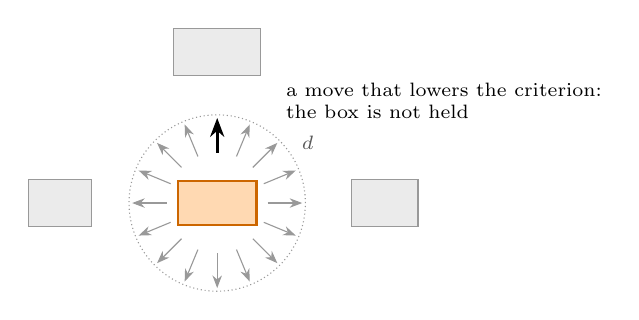
\begin{tikzpicture}[x=1cm,y=1cm,line width=0.4pt,font=\footnotesize]
  \draw[fill=black!8,draw=black!40] (-0.55,1.62) rectangle (0.55,2.22);
  \draw[fill=black!8,draw=black!40] (1.70,-0.30) rectangle (2.55,0.30);
  \draw[fill=black!8,draw=black!40] (-2.40,-0.30) rectangle (-1.60,0.30);
  \draw[densely dotted,black!40] (0,0) circle (1.12);
  \foreach \a in {0,22.5,45,67.5,112.5,135,157.5,180,202.5,225,247.5,270,292.5,315,337.5}{
    \draw[-{Stealth[length=1.6mm]},black!40] (\a:0.64) -- (\a:1.08);}
  \draw[-{Stealth[length=2.4mm]},black,line width=1pt] (90:0.64) -- (90:1.08);
  \draw[fill=orange!30,draw=orange!80!black,line width=0.8pt]
       (-0.5,-0.28) rectangle (0.5,0.28);
  \node[font=\scriptsize,black!65] at (33.75:1.38) {$d$};
  \node[anchor=west,font=\scriptsize,align=left] at (0.75,1.30)
       {a move that lowers the criterion:\\the box is not held};
\end{tikzpicture}
\caption{The test, one box and one criterion. The box is moved a distance $d$, two per
cent of the drawing's width, in each of sixteen exact directions, and the criterion is
recomputed. If some move lowers it (the dark arrow), the box is not held; if every move
raises it, the box is \emph{held}.}
\label{fig:test}
\end{figure}


\paragraph{The energy.} A layout of a graph with $N$ nodes is a point
$x \in \mathbb{R}^{2N}$, two coordinates per node, the boxes' sizes held fixed. An
aesthetic energy is
\begin{equation}
E_w(x) = \sum_{k=1}^{K} w_k\, T_k(x), \qquad w_k \ge 0,
\end{equation}
where each term $T_k$ is a quantity to be made small. Multicriteria layout is the choice
of the $T_k$ and the $w_k$ \cite{dh96, purchase02}.

\paragraph{Held.} A point $x$ is a local minimum of $E$ if $E(y) \ge E(x)$ for every $y$
within some distance of $x$. Two terms here are not differentiable, crossings being a
count and overlap having corners where boxes touch, so the test uses no gradient. Fix a
radius $d$ and a set $V$ of sixteen equally spaced unit directions. For node $i$ and
direction $v$ let $x + d\,v^{(i)}$ be the layout with node $i$ moved by $d$ along $v$ and
every other node fixed (Figure~\ref{fig:test}). Node $i$ is \emph{held} at radius $d$ if
\begin{equation}
E(x + d\,v^{(i)}) \ge E(x) \quad \text{for every } v \in V,
\label{eq:held}
\end{equation}
and the estimand is
\begin{equation}
q_d(x) = \frac{1}{N}\,\#\{\,i : \text{node } i \text{ is held at radius } d\,\}.
\label{eq:q}
\end{equation}
$q_d = 1$ says the layout is a local minimum of $E$ over single-node moves of length $d$;
for smooth $E$ and small $d$ it says $\nabla E(x) = 0$ to within the resolution of $V$. A
person in a diagram editor moves one box at a time, so single-node moves are the editor's
own move set, and equation~\eqref{eq:held} compares two energies, so it is defined for
every term. Evaluated per term it separates the criteria a layout satisfies from those it
does not. The primary radius is $d = 0.02$ of the drawing width, about one grid step in
the editors of Section~\ref{sec:corpora}; a move that lowers the energy by less than
$10^{-12}$ of its value is a tie. The test is deterministic: no seed, no budget.

\paragraph{What $q$ counts.} A held fraction means different things for terms of
different shape. For a smooth term near a minimum with gradient $g$ and curvature
$\lambda$, a node is held when $|g| < d\lambda/2$: $q$ reads how near the minimum is. For
a count (crossings) or a step function of position (gridiness, below), the term is flat
almost everywhere and a node is held wherever no move of length $d$ changes it: $q$ reads
how much of the layout the term has stopped acting on, so the term's value is reported
beside it. For a term with a corner at exact coincidence (the alignment term A1 below), a
node is held when it sits within about $d/2$ of sharing a coordinate with another node,
and it is free to slide along that row or column: $q$ counts boxes pinned in one
coordinate. The results report, beside $q$, the median best decrease a single move finds
as a fraction of the term's value, and the share of diagrams in which any box has an
improving move at all.

\paragraph{The inverse problem.} Given layouts $x^{(1)}, \dots, x^{(G)}$ that people
accepted, inverse optimisation asks for the weights $w$ under which they are nearest to
stationary \cite{keshavarz11, chan19}. With the directional differences
$D_{iv} T_k = T_k(x + d\,v^{(i)}) - T_k(x)$ in hand, node $i$ is held under $w$ exactly
when $\sum_k w_k D_{iv} T_k \ge 0$ for all $v$, a set of linear inequalities in $w$. The
residual is the smallest total violation over $w$ on the simplex, a linear program, and it
is zero only if some weighting makes the layout a local minimum. Two properties of that
program decide what a fit can return. A term with $D_{iv} T_k < 0$ for some $v$ at almost
every node cannot take positive weight without violating the inequalities at those nodes.
And a term every layout satisfies exactly, with $D_{iv} T_k \ge 0$ everywhere, is a
zero-residual vertex on its own: the program returns all weight on it and learns nothing.
The second is the degeneracy Ng and Russell \cite{ng00} state for inverse reinforcement
learning, where a zero reward makes every policy optimal; their repair and its successors
add a margin \cite{ratliff06} or a noise model under which demonstrations are only
near-optimal \cite{ziebart08, aswani18}. Neither rescues a term of the first kind: a term
some direction lowers at almost every node carries no weight under any margin, and the
sweep of Section~\ref{sec:results} measures that directly.

\paragraph{The reference length.} The length and stress terms compare distances with a
reference $L$. Fixed at the layout's median edge length, $L$ is in general not the scale
at which the term is least for that layout, so at a true minimum every node still has a
scaling direction that lowers the term: \texttt{neato}'s converged stress layouts read
$q = 0.07$ to $0.12$ under their own criterion. $L$ is therefore the value at which the
term is least for the layout as loaded, $\sum \ell^2 / \sum \ell$ over edges for length and
the same over $\|x_i - x_j\| / \delta_{ij}$ for stress, fixed before any move; the
converged layouts are then held at $1.00$. This is the scale-normalised stress of Smelser,
Miller and Kobourov \cite{smelser24}, whose minimiser is in closed form, and of Ahmed et
al.\ \cite{ahmed24} for the graph stress used here; under scale-sensitive stress they find
a random layout ranked ahead of \texttt{neato} on nearly every graph of two benchmarks,
and fitting $L$ is the known repair. The median and $1/\sqrt{N}$ are sensitivities
(Appendix~\ref{app:reference}).

\paragraph{The controls.} A test that can only succeed is not a test. The
\emph{converged reference}: $q_d$ on a layout a descent has converged on must be near
one, or the test lacks power for that energy. \texttt{neato}'s layouts are the reference
for stress, and the end point of an uncapped descent from each hand layout is the
reference for every summed energy (median $q$ 1.00 in every corpus,
Appendix~\ref{app:descent}). The \emph{tool controls}: the same graphs with the same box
sizes and edge directions laid out by \texttt{neato} (stress, \texttt{-Gstart=1}, boxes
left where they overlap), \texttt{prism} (\texttt{neato} followed by its overlap removal),
\texttt{dot} (layered) and ELK layered 0.12.0 \cite{schulze14}, the engine the BPMN
editors run; a check in the binary confirms each control is the same graphs. The
\emph{null}: a uniform random layout of the same graph in the same bounding box, and for
the alignment term a random layout snapped to the same grid as the drawing.

\paragraph{Terms.} With $n$ nodes, $m$ edges, box $i$ of width $w_i$ and height $h_i$, and
$L$ fitted to the layout under test:

\begin{center}\footnotesize
\begin{tabular}{lp{7.6cm}p{2.6cm}}
\toprule
term & definition & zero when \\
\midrule
$T_C$ crossings & proper crossings between segments of two routes with no shared endpoint, $/m$ & planar \\
$T_O$ overlap & overlap area of boxes $/$ total box area & no overlap \\
$T_L$ length uniformity & mean over edges of $((\ell - L)/L)^2$ & all edges of length $L$ \\
$T_S$ stress & $\sum_{i<j} (\|x_i - x_j\| - L\,\delta_{ij})^2 / \delta_{ij}^2$, $\delta_{ij}$ the graph distance & distances proportional \\
$T_R$ orthogonality & mean over edges of the length-weighted mean over its segments of $\min(|\Delta x|,|\Delta y|)/(|\Delta x|+|\Delta y|)$ & routes axis-aligned \\
$T_A$ alignment & A1: mean over nodes of the distance to the nearest other node along whichever axis is nearer & every node in a row or column \\
gridiness & $1 -$ fraction of nodes in an alignment of $\ge 3$ (tolerance 0.005), HOLA's definition \cite{hola16}, a step & every node aligned \\
$T_N$ node--edge & squared shortfall of node to foreign route distance below $(w+h)/4$ & none within \\
$T_F$ flow & mean over directed edges of the backward component along the reading direction $u$, over length & no edge runs back \\
\bottomrule
\end{tabular}
\end{center}

The base energy is $T_C + T_O + T_L$ at weights $(1,1,1)$, the form of Davidson and
Harel's simulated annealing \cite{dh96} and of the multicriteria tradition since
\cite{ahmed20}; stress \cite{kamada89, gansner05}, which force-directed tools and
\texttt{neato} minimise, is the second base energy. $T_R$, $T_A$ and $T_N$ are the
candidates for what the base energy misses. A1 has a corner at exact alignment; a smooth
Gaussian form, A3 with width 0.02, is the sensitivity and holds a third to half of what
the corner holds (Section~\ref{sec:results}). The reading direction $u$ is the axis
direction under which $T_F$ is least for the layout as loaded, fixed before any move,
the same rule as for $L$.

\paragraph{Routes.} An edge is the polyline the file stores: the attachment point on the
source box, the interior waypoints, the attachment point on the target box; where the
file stores nothing it is the chord between the centres. Crossings, orthogonality and
node--edge separation are evaluated on the route; length and stress on the centres. When
a node moves its attachment points move with it and the waypoints stay. A waypoint is
stored on 0.29, 0.07 and 0.33 of the edges by corpus, and only the BPMN routes are
orthogonal: 0.88 of them are axis-aligned at every segment, against 0.01 in the two
biological formats. The chords are the sensitivity, and no verdict moves under them.

\paragraph{Fitting.} Weights on the simplex, the linear program above over every node and
direction of a corpus (about 120,000 inequalities, HiGHS), the residual its value per
node. Because the residual depends on the terms' scales and $q$ does not, $q$ under the
fitted weights is reported beside it, on the fitting diagrams and held out under
$5 \times 2$ cross-validation (five seeded halvings, each half fitted and scored on the
other). The sweep, $q$ as the weight on one term grows from 0 with the rest on crossings
and overlap, is the test of whether any positive weight on that term can be carried.

\paragraph{Statistics.} The unit of inference is the diagram. Every median carries a 95\%
bootstrap interval over diagrams (1,000 resamples). An interval of [0.00, 0.00] or [1.00,
1.00] is a pileup at the boundary, so the share of diagrams at exactly that value is given
where it matters. Paired comparisons of hand against tool on one criterion are
Hodges--Lehmann shifts with distribution-free 95\% intervals, Holm-corrected within a
corpus (Appendix~\ref{app:paired}); equivalence claims are read off the sweep, never off a
failure to reject.

\paragraph{The instrument.} The directional test, the terms and the parsers are C in the
repository under \texttt{example/diagrams}. The descents come from \texttt{cjitter}, a C
library of stochastic searches over a box of real variables, byte-reproducible from a seed
on every platform, with uniform sampling at the same budget as its built-in control.

\section{The corpora}\label{sec:corpora}

Three collections of diagrams whose node coordinates a person chose, from three
communities with different authoring tools, all redistributable, and two collections of
drawings made for their own sake.

\begin{center}\footnotesize
\begin{tabular}{llrrrl}
\toprule
corpus & made in & files & 15--40 nodes & used & median $m/n$ \\
\midrule
WikiPathways GPML, \emph{Homo sapiens} \cite{agrawal24} & PathVisio & 1,016 & 305 & 305 & 1.06 \\
Reactome SBGN-ML \cite{fabregat18} & curation tool & 1,382 & 248 & 248 & 1.04 \\
BPMN Academic Initiative \cite{kunze11, sola23} & Signavio & 13,435 & 6,723 & 300 & 1.11 \\
HOLA formative drawings \cite{hola16} & study tool & 136 & (4--13) & 136 & \\
GD Collection \cite{gdcoll25} & mixed & 4,890 & 1,072 & 1,072 & \\
\bottomrule
\end{tabular}
\end{center}

The first three are working documents: Reactome diagrams are laid out by curators,
WikiPathways pathways are drawn in PathVisio, and the BPMN models are students' work in
Signavio. Nobody was asked to draw nicely, and the three tools share no layout code. A
diagram enters as its largest connected component of 15 to 40 nodes, container glyphs
(SBGN compartments, BPMN pools and lanes) not being nodes and SBGN process glyphs being
nodes; each layout is rescaled uniformly so that its bounding box fits the unit square, box
sizes with it. The BPMN archive is used only where every edge is a BPMN flow or
association, 13,435 of 21,784 parsed models, and the corpus is a seeded random 300 of the
6,723 in the band; the first 300 by model id, the sample the study was planned on, sits
at the 99th percentile of random samples on alignment and is retired to
Appendix~\ref{app:bpmn}. Two WikiPathways files carry coordinates converted from Reactome
\cite{bohler16} and are dropped; deduplication and clustering by drawer move no median
(Appendix~\ref{app:corpus}).

The two further collections are drawings, not working diagrams. HOLA's formative
corpus is 17 participants each laying out the same 8 abstract graphs in a study tool,
136 drawings of 4 to 13 nodes, scraped from the study's published SVGs. The GD
Collection is 4,890 figures harvested from 27 editions of this field's proceedings, of
which 1,072 have a largest component in the band; its provenance is not per drawing, its
authors' audit reproduces 69\% of figures exactly, edge directions and box sizes are
absent, so only the terms needing neither are run on it.

How the coordinates were made matters for the alignment criterion. Of the raw
coordinates, 17\% are integers in WikiPathways, 67\% in Reactome and 63\% in BPMN; the
fraction of boxes sharing an exact $x$ with another box is 0.37, 0.06 and 0.41, an exact
$y$ 0.29, 0.12 and 0.77, and either 0.54, 0.17 and 0.87, the figures the alignment row of
Section~\ref{sec:results} should be read against. In WikiPathways exact alignment is
twice as common as integer coordinates, so it is not a rounding grid's act. PathVisio and
the BPMN editors draw a snap-to-object guide on every drag; Reactome's curation tool does
not. Section~\ref{sec:alternatives} takes this up.

\section{What the coordinates hold}\label{sec:results}

\begin{figure}[t]\centering
\begin{tabular}{@{}c@{\hspace{3pt}}c@{\hspace{3pt}}c@{\hspace{3pt}}c@{}}
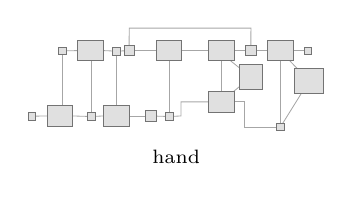
\begin{tikzpicture}[x=1cm,y=1cm,line width=0.3pt]
\draw[gray!70] (0.439,1.016) -- (0.632,1.019);
\draw[gray!70] (0.439,0.319) -- (0.439,1.016);
\draw[gray!70] (2.686,0.798) -- (2.572,0.889);
\draw[gray!70] (1.950,1.019) -- (2.292,1.019);
\draw[gray!70] (2.617,1.019) -- (2.829,1.019);
\draw[gray!70] (2.454,0.498) -- (2.454,0.889);
\draw[gray!70] (2.607,0.498) -- (2.686,0.563);
\draw[gray!70] (1.283,1.019) -- (1.624,1.019);
\draw[gray!70] (2.829,1.019) -- (2.830,1.305) -- (1.284,1.305) -- (1.283,1.019);
\draw[gray!70] (1.126,1.012) -- (1.283,1.019);
\draw[gray!70] (1.794,0.889) -- (1.794,0.182);
\draw[gray!70] (2.829,1.019) -- (3.040,1.019);
\draw[gray!70] (3.366,1.019) -- (3.558,1.019);
\draw[gray!70] (3.324,0.889) -- (3.418,0.791);
\draw[gray!70] (3.203,0.889) -- (3.203,0.046);
\draw[gray!70] (3.470,0.475) -- (3.203,0.046);
\draw[gray!70] (0.957,1.019) -- (1.126,1.012);
\draw[gray!70] (0.801,0.889) -- (0.801,0.182);
\draw[gray!70] (1.126,0.319) -- (1.126,1.012);
\draw[gray!70] (0.049,0.186) -- (0.241,0.189);
\draw[gray!70] (0.566,0.189) -- (0.801,0.182);
\draw[gray!70] (0.801,0.182) -- (0.957,0.189);
\draw[gray!70] (1.283,0.189) -- (1.559,0.189);
\draw[gray!70] (1.794,0.182) -- (1.942,0.189) -- (1.942,0.368) -- (2.292,0.368);
\draw[gray!70] (1.559,0.189) -- (1.794,0.182);
\draw[gray!70] (2.617,0.368) -- (2.744,0.368) -- (2.744,0.046) -- (3.203,0.046);
\draw[fill=black!12,draw=black!55] (0.391,0.967) rectangle (0.488,1.064);
\draw[fill=black!12,draw=black!55] (2.292,0.889) rectangle (2.617,1.149);
\draw[fill=black!12,draw=black!55] (2.686,0.524) rectangle (2.972,0.840);
\draw[fill=black!12,draw=black!55] (1.217,0.954) rectangle (1.348,1.084);
\draw[fill=black!12,draw=black!55] (1.624,0.889) rectangle (1.950,1.149);
\draw[fill=black!12,draw=black!55] (2.764,0.954) rectangle (2.894,1.084);
\draw[fill=black!12,draw=black!55] (3.040,0.889) rectangle (3.366,1.149);
\draw[fill=black!12,draw=black!55] (3.512,0.973) rectangle (3.604,1.064);
\draw[fill=black!12,draw=black!55] (3.385,0.475) rectangle (3.750,0.791);
\draw[fill=black!12,draw=black!55] (0.632,0.889) rectangle (0.957,1.149);
\draw[fill=black!12,draw=black!55] (1.077,0.964) rectangle (1.175,1.061);
\draw[fill=black!12,draw=black!55] (0.000,0.137) rectangle (0.098,0.234);
\draw[fill=black!12,draw=black!55] (0.241,0.059) rectangle (0.566,0.319);
\draw[fill=black!12,draw=black!55] (0.752,0.133) rectangle (0.850,0.231);
\draw[fill=black!12,draw=black!55] (0.957,0.059) rectangle (1.283,0.319);
\draw[fill=black!12,draw=black!55] (1.745,0.133) rectangle (1.842,0.231);
\draw[fill=black!12,draw=black!55] (2.292,0.238) rectangle (2.617,0.498);
\draw[fill=black!12,draw=black!55] (1.494,0.124) rectangle (1.624,0.254);
\draw[fill=black!12,draw=black!55] (3.158,0.000) rectangle (3.249,0.091);
\node[anchor=north,font=\scriptsize] at (1.88,-0.12) {hand};
\end{tikzpicture}
&
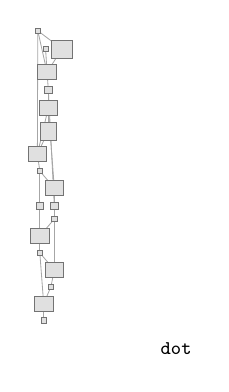
\begin{tikzpicture}[x=1cm,y=1cm,line width=0.3pt]
\draw[gray!70] (0.290,0.465) -- (0.333,0.680);
\draw[gray!70] (0.198,0.250) -- (0.290,0.465);
\draw[gray!70] (0.257,2.443) -- (0.257,2.737);
\draw[gray!70] (0.333,1.719) -- (0.257,2.737);
\draw[gray!70] (0.257,2.737) -- (0.257,2.964);
\draw[gray!70] (0.118,2.149) -- (0.257,2.737);
\draw[gray!70] (0.118,2.149) -- (0.257,2.443);
\draw[gray!70] (0.333,1.492) -- (0.333,1.719);
\draw[gray!70] (0.257,2.964) -- (0.333,1.492);
\draw[gray!70] (0.333,1.325) -- (0.333,1.492);
\draw[gray!70] (0.333,1.719) -- (0.149,1.934);
\draw[gray!70] (0.257,2.964) -- (0.241,3.190);
\draw[gray!70] (0.241,3.190) -- (0.222,3.484);
\draw[gray!70] (0.241,3.190) -- (0.430,3.484);
\draw[gray!70] (0.241,3.190) -- (0.123,3.717);
\draw[gray!70] (0.430,3.484) -- (0.123,3.717);
\draw[gray!70] (0.333,0.680) -- (0.333,1.325);
\draw[gray!70] (0.333,0.680) -- (0.149,0.895);
\draw[gray!70] (0.149,1.110) -- (0.333,1.325);
\draw[gray!70] (0.198,0.035) -- (0.198,0.250);
\draw[gray!70] (0.198,0.250) -- (0.149,0.895);
\draw[gray!70] (0.149,0.895) -- (0.149,1.110);
\draw[gray!70] (0.149,1.110) -- (0.149,1.492);
\draw[gray!70] (0.149,1.934) -- (0.118,2.149);
\draw[gray!70] (0.149,1.492) -- (0.149,1.934);
\draw[gray!70] (0.118,2.149) -- (0.123,3.717);
\draw[fill=black!12,draw=black!55] (0.255,0.430) rectangle (0.326,0.501);
\draw[fill=black!12,draw=black!55] (0.139,2.642) rectangle (0.375,2.831);
\draw[fill=black!12,draw=black!55] (0.154,2.328) rectangle (0.361,2.557);
\draw[fill=black!12,draw=black!55] (0.286,1.445) rectangle (0.380,1.540);
\draw[fill=black!12,draw=black!55] (0.215,1.625) rectangle (0.451,1.814);
\draw[fill=black!12,draw=black!55] (0.210,2.916) rectangle (0.305,3.011);
\draw[fill=black!12,draw=black!55] (0.123,3.096) rectangle (0.359,3.285);
\draw[fill=black!12,draw=black!55] (0.189,3.451) rectangle (0.255,3.517);
\draw[fill=black!12,draw=black!55] (0.298,3.370) rectangle (0.562,3.599);
\draw[fill=black!12,draw=black!55] (0.215,0.586) rectangle (0.451,0.774);
\draw[fill=black!12,draw=black!55] (0.298,1.289) rectangle (0.368,1.360);
\draw[fill=black!12,draw=black!55] (0.163,0.000) rectangle (0.234,0.071);
\draw[fill=black!12,draw=black!55] (0.080,0.156) rectangle (0.316,0.345);
\draw[fill=black!12,draw=black!55] (0.113,0.859) rectangle (0.184,0.930);
\draw[fill=black!12,draw=black!55] (0.031,1.015) rectangle (0.267,1.204);
\draw[fill=black!12,draw=black!55] (0.113,1.899) rectangle (0.184,1.969);
\draw[fill=black!12,draw=black!55] (0.000,2.054) rectangle (0.236,2.243);
\draw[fill=black!12,draw=black!55] (0.102,1.445) rectangle (0.196,1.540);
\draw[fill=black!12,draw=black!55] (0.090,3.684) rectangle (0.156,3.750);
\node[anchor=north,font=\scriptsize] at (1.88,-0.12) {\texttt{dot}};
\end{tikzpicture}
&
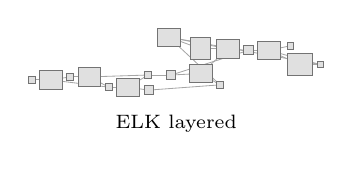
\begin{tikzpicture}[x=1cm,y=1cm,line width=0.3pt]
\draw[gray!70] (0.534,0.245) -- (0.779,0.245);
\draw[gray!70] (0.288,0.207) -- (0.534,0.245);
\draw[gray!70] (2.192,0.601) -- (2.538,0.601);
\draw[gray!70] (2.192,0.288) -- (2.538,0.601);
\draw[gray!70] (2.538,0.601) -- (2.798,0.582);
\draw[gray!70] (1.788,0.750) -- (2.538,0.601);
\draw[gray!70] (1.788,0.750) -- (2.192,0.601);
\draw[gray!70] (1.817,0.269) -- (2.192,0.288);
\draw[gray!70] (2.798,0.582) -- (1.817,0.269);
\draw[gray!70] (1.524,0.269) -- (1.817,0.269);
\draw[gray!70] (2.192,0.288) -- (2.438,0.144);
\draw[gray!70] (2.798,0.582) -- (3.058,0.582);
\draw[gray!70] (3.058,0.582) -- (3.329,0.640);
\draw[gray!70] (3.058,0.582) -- (3.450,0.402);
\draw[gray!70] (3.058,0.582) -- (3.710,0.402);
\draw[gray!70] (3.450,0.402) -- (3.710,0.402);
\draw[gray!70] (0.779,0.245) -- (1.524,0.269);
\draw[gray!70] (0.779,0.245) -- (1.024,0.115);
\draw[gray!70] (1.269,0.115) -- (1.524,0.269);
\draw[gray!70] (0.043,0.207) -- (0.288,0.207);
\draw[gray!70] (0.288,0.207) -- (1.024,0.115);
\draw[gray!70] (1.024,0.115) -- (1.269,0.115);
\draw[gray!70] (1.269,0.115) -- (1.529,0.077);
\draw[gray!70] (2.438,0.144) -- (1.788,0.750);
\draw[gray!70] (1.529,0.077) -- (2.438,0.144);
\draw[gray!70] (1.788,0.750) -- (3.710,0.402);
\draw[fill=black!12,draw=black!55] (0.490,0.202) rectangle (0.577,0.288);
\draw[fill=black!12,draw=black!55] (2.394,0.486) rectangle (2.683,0.717);
\draw[fill=black!12,draw=black!55] (2.065,0.462) rectangle (2.319,0.741);
\draw[fill=black!12,draw=black!55] (1.760,0.212) rectangle (1.875,0.327);
\draw[fill=black!12,draw=black!55] (2.048,0.173) rectangle (2.337,0.404);
\draw[fill=black!12,draw=black!55] (2.740,0.525) rectangle (2.856,0.640);
\draw[fill=black!12,draw=black!55] (2.913,0.467) rectangle (3.202,0.698);
\draw[fill=black!12,draw=black!55] (3.288,0.600) rectangle (3.369,0.680);
\draw[fill=black!12,draw=black!55] (3.288,0.262) rectangle (3.612,0.542);
\draw[fill=black!12,draw=black!55] (0.635,0.130) rectangle (0.923,0.361);
\draw[fill=black!12,draw=black!55] (1.481,0.226) rectangle (1.567,0.312);
\draw[fill=black!12,draw=black!55] (0.000,0.163) rectangle (0.087,0.250);
\draw[fill=black!12,draw=black!55] (0.144,0.091) rectangle (0.433,0.322);
\draw[fill=black!12,draw=black!55] (0.981,0.072) rectangle (1.067,0.159);
\draw[fill=black!12,draw=black!55] (1.125,0.000) rectangle (1.413,0.231);
\draw[fill=black!12,draw=black!55] (2.394,0.101) rectangle (2.481,0.188);
\draw[fill=black!12,draw=black!55] (1.644,0.635) rectangle (1.933,0.865);
\draw[fill=black!12,draw=black!55] (1.471,0.019) rectangle (1.587,0.135);
\draw[fill=black!12,draw=black!55] (3.669,0.362) rectangle (3.750,0.442);
\node[anchor=north,font=\scriptsize] at (1.88,-0.12) {ELK layered};
\end{tikzpicture}
&
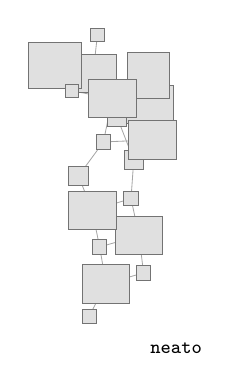
\begin{tikzpicture}[x=1cm,y=1cm,line width=0.3pt]
\draw[gray!70] (1.466,0.642) -- (1.409,1.115);
\draw[gray!70] (0.989,0.501) -- (1.466,0.642);
\draw[gray!70] (1.528,3.147) -- (1.542,2.781);
\draw[gray!70] (1.579,2.330) -- (1.542,2.781);
\draw[gray!70] (1.542,2.781) -- (1.130,2.620);
\draw[gray!70] (1.069,2.855) -- (1.542,2.781);
\draw[gray!70] (1.069,2.855) -- (1.528,3.147);
\draw[gray!70] (1.342,2.074) -- (1.579,2.330);
\draw[gray!70] (1.130,2.620) -- (1.342,2.074);
\draw[gray!70] (1.307,1.584) -- (1.342,2.074);
\draw[gray!70] (1.579,2.330) -- (0.957,2.304);
\draw[gray!70] (1.130,2.620) -- (0.825,3.170);
\draw[gray!70] (0.825,3.170) -- (0.881,3.665);
\draw[gray!70] (0.825,3.170) -- (0.339,3.274);
\draw[gray!70] (0.825,3.170) -- (0.555,2.954);
\draw[gray!70] (0.339,3.274) -- (0.555,2.954);
\draw[gray!70] (1.409,1.115) -- (1.307,1.584);
\draw[gray!70] (1.409,1.115) -- (0.909,0.970);
\draw[gray!70] (0.813,1.436) -- (1.307,1.584);
\draw[gray!70] (0.776,0.091) -- (0.989,0.501);
\draw[gray!70] (0.989,0.501) -- (0.909,0.970);
\draw[gray!70] (0.909,0.970) -- (0.813,1.436);
\draw[gray!70] (0.813,1.436) -- (0.640,1.872);
\draw[gray!70] (0.957,2.304) -- (1.069,2.855);
\draw[gray!70] (0.640,1.872) -- (0.957,2.304);
\draw[gray!70] (1.069,2.855) -- (0.555,2.954);
\draw[fill=black!12,draw=black!55] (1.375,0.551) rectangle (1.557,0.733);
\draw[fill=black!12,draw=black!55] (1.239,2.539) rectangle (1.845,3.024);
\draw[fill=black!12,draw=black!55] (1.262,2.853) rectangle (1.795,3.441);
\draw[fill=black!12,draw=black!55] (1.220,1.953) rectangle (1.463,2.195);
\draw[fill=black!12,draw=black!55] (1.276,2.087) rectangle (1.882,2.572);
\draw[fill=black!12,draw=black!55] (1.009,2.499) rectangle (1.251,2.741);
\draw[fill=black!12,draw=black!55] (0.522,2.927) rectangle (1.128,3.412);
\draw[fill=black!12,draw=black!55] (0.796,3.580) rectangle (0.966,3.750);
\draw[fill=black!12,draw=black!55] (0.000,2.980) rectangle (0.679,3.568);
\draw[fill=black!12,draw=black!55] (1.106,0.873) rectangle (1.712,1.358);
\draw[fill=black!12,draw=black!55] (1.216,1.493) rectangle (1.398,1.675);
\draw[fill=black!12,draw=black!55] (0.685,0.000) rectangle (0.867,0.182);
\draw[fill=black!12,draw=black!55] (0.686,0.259) rectangle (1.292,0.744);
\draw[fill=black!12,draw=black!55] (0.818,0.879) rectangle (1.000,1.061);
\draw[fill=black!12,draw=black!55] (0.510,1.193) rectangle (1.116,1.678);
\draw[fill=black!12,draw=black!55] (0.866,2.213) rectangle (1.048,2.395);
\draw[fill=black!12,draw=black!55] (0.766,2.612) rectangle (1.372,3.097);
\draw[fill=black!12,draw=black!55] (0.518,1.751) rectangle (0.761,1.994);
\draw[fill=black!12,draw=black!55] (0.470,2.870) rectangle (0.640,3.039);
\node[anchor=north,font=\scriptsize] at (1.88,-0.12) {\texttt{neato}};
\end{tikzpicture}
\end{tabular}
\caption{The same graph, the same box sizes, four layouts. The hand drawing and the two
layered tools share the profile the test reads: held under overlap, free under length and
stress. \texttt{neato} minimises stress and is the control that gives the test its power,
held at 1.00 under stress where every hand layout reads 0.00. The tool layouts carry no
waypoints, so their edges are drawn as chords.}
\label{fig:tools}
\end{figure}


The tables are from one deterministic pass over the corpora
(\texttt{results/run\_all.sh}; commit, versions, seeds and corpus hashes in
\texttt{results/manifest.txt}); the BPMN sample runs by the same script with
\texttt{--corpora BPMN:bpmnr}.

\paragraph{Each criterion alone.} $q_{0.02}$ on the hand layout with its 95\% interval,
on \texttt{neato}, \texttt{dot} and ELK layouts of the same graphs, and on a uniform
random layout; in parentheses the median value of the term at the layout, 0 when
satisfied. \texttt{prism}, the A3 kernel and the summed energies are in
Appendix~\ref{app:sums}.

\begin{center}\scriptsize\setlength{\tabcolsep}{3.5pt}
\begin{tabular}{llrrrrr}
\toprule
corpus & term & hand & \texttt{neato} & \texttt{dot} & ELK & random \\
\midrule
WikiPathways & crossings & 1.00 [1.00, 1.00] (0.000) & 1.00 (0.000) & 1.00 (0.029) & 1.00 (0.036) & 0.67 \\
& overlap & 1.00 [1.00, 1.00] (0.000) & 0.60 (0.030) & 1.00 (0.000) & 1.00 (0.000) & 0.67 \\
& length & 0.00 [0.00, 0.00] (0.219) & 0.24 (0.011) & 0.00 (0.241) & 0.00 (0.127) & 0.00 \\
& stress & 0.00 [0.00, 0.00] (0.217) & 1.00 (0.042) & 0.00 (0.201) & 0.00 (0.241) & 0.00 \\
& orthogonality & 0.19 [0.18, 0.21] (0.157) & 0.00 (0.280) & 0.19 (0.244) & 0.19 (0.158) & 0.00 \\
& alignment A1 & 0.52 [0.48, 0.54] (0.003) & 0.06 (0.011) & 1.00 (0.000) & 0.57 (0.001) & 0.07 \\
& gridiness & 0.87 [0.84, 0.89] (0.424) & 0.78 (1.000) & 1.00 (0.125) & 0.76 (0.200) & \\
& node--edge & 0.88 [0.86, 0.90] (0.004) & 0.89 (0.000) & 0.78 (0.011) & 0.74 (0.016) & 0.12 \\
& flow & 0.59 [0.56, 0.62] (0.131) & 0.50 (0.211) & 1.00 (0.000) & 1.00 (0.000) & 0.41 \\
\midrule
Reactome & crossings & 1.00 [1.00, 1.00] (0.000) & 1.00 (0.000) & 1.00 (0.056) & 1.00 (0.066) & 0.61 \\
& overlap & 1.00 [1.00, 1.00] (0.000) & 0.76 (0.022) & 1.00 (0.000) & 1.00 (0.000) & 0.67 \\
& length & 0.00 [0.00, 0.00] (0.234) & 0.35 (0.005) & 0.00 (0.232) & 0.00 (0.205) & 0.00 \\
& stress & 0.00 [0.00, 0.00] (0.212) & 1.00 (0.034) & 0.00 (0.177) & 0.00 (0.197) & 0.00 \\
& orthogonality & 0.17 [0.15, 0.18] (0.193) & 0.00 (0.277) & 0.15 (0.256) & 0.12 (0.203) & 0.00 \\
& alignment A1 & 0.21 [0.19, 0.24] (0.004) & 0.06 (0.009) & 1.00 (0.000) & 0.42 (0.002) & 0.06 \\
& gridiness & 0.65 [0.62, 0.68] (0.640) & 0.77 (1.000) & 0.95 (0.176) & 0.74 (0.306) & \\
& node--edge & 1.00 [0.94, 1.00] (0.000) & 0.93 (0.000) & 0.80 (0.007) & 0.75 (0.021) & 0.11 \\
& flow & 0.62 [0.60, 0.67] (0.096) & 0.45 (0.217) & 1.00 (0.000) & 1.00 (0.000) & 0.36 \\
\midrule
BPMN & crossings & 1.00 [1.00, 1.00] (0.000) & 1.00 (0.000) & 1.00 (0.000) & 1.00 (0.000) & 0.58 \\
& overlap & 1.00 [1.00, 1.00] (0.000) & 0.41 (0.071) & 1.00 (0.000) & 1.00 (0.000) & 0.63 \\
& length & 0.00 [0.00, 0.00] (0.284) & 0.40 (0.005) & 0.00 (0.222) & 0.00 (0.250) & 0.00 \\
& stress & 0.00 [0.00, 0.00] (0.197) & 1.00 (0.016) & 0.00 (0.152) & 0.00 (0.175) & 0.00 \\
& orthogonality & 0.73 [0.71, 0.75] (0.011) & 0.00 (0.277) & 0.27 (0.169) & 0.25 (0.145) & 0.00 \\
& alignment A1 & 0.85 [0.82, 0.89] (0.001) & 0.06 (0.011) & 1.00 (0.000) & 0.59 (0.001) & 0.07 \\
& gridiness & 0.95 [0.94, 0.96] (0.188) & 0.79 (1.000) & 0.81 (0.238) & 0.67 (0.279) & \\
& node--edge & 1.00 [1.00, 1.00] (0.000) & 1.00 (0.000) & 0.86 (0.001) & 0.79 (0.011) & 0.11 \\
& flow & 0.86 [0.83, 0.88] (0.041) & 0.62 (0.120) & 1.00 (0.000) & 1.00 (0.000) & 0.26 \\
\bottomrule
\end{tabular}
\end{center}

Read down a hand column. Overlap holds every box at value zero, as it does in every tool
layout that removes overlaps. Length and stress hold no box of the median hand diagram,
and 0.87 to 0.92 of diagrams sit at exactly 0.00; \texttt{neato}'s stress layouts are held
at 1.00 under the same test, so the zero is the layout's and not the test's. The random
layouts read 0.00 too, as do \texttt{dot} and ELK, which are layered and price no
distance: at this radius no layout is stationary under a distance term except a
minimiser's converged output, so the distance result separates optimisers from everyone
and the hand layouts stand with the layered engines. Hand and \texttt{neato} part
furthest on alignment. The gridiness value puts 58, 36 and 81 per cent of hand-placed
boxes in an alignment of three or more, none of \texttt{neato}'s, and 88, 82 and 76 per
cent of \texttt{dot}'s, since a layer is a row; the gridiness $q$ on \texttt{neato}'s
layouts is the step's flatness, so alignment is compared on the value, with the A1 hold
beside it as the count a fit needs. The A1 hold tracks the exact-tie fractions of
Section~\ref{sec:corpora} (0.54, 0.17, 0.87) to within a few points, as a corner term
should. Alignment does not hold the most boxes: node--edge separation holds 0.88 to 1.00
and crossings and overlap hold every box. What separates alignment from those three is
that the base energy prices them and does not price it.

\paragraph{What the zeros mean.} Beside each $q$ the table gives \emph{dec}, the median
over diagrams of the mean best decrease a single move finds as a fraction of the term's
value, and \emph{active}, the share of diagrams in which any box has an improving move.

\begin{center}\small
\begin{tabular}{@{}lccc@{\hspace{14pt}}ccc@{\hspace{14pt}}ccc@{}}
\toprule
& \multicolumn{3}{c}{WikiPathways} & \multicolumn{3}{c}{Reactome} & \multicolumn{3}{c}{BPMN} \\
\cmidrule(r){2-4}\cmidrule(r){5-7}\cmidrule{8-10}
term & $q$ & dec & active & $q$ & dec & active & $q$ & dec & active \\
\midrule
crossings      & 1.00 & 0.000 & 30\% & 1.00 & 0.000 & 20\% & 1.00 & 0.000 & 3\% \\
overlap        & 1.00 & 0.000 & 18\% & 1.00 & 0.000 & 5\%  & 1.00 & 0.000 & 8\% \\
node--edge     & 0.88 & 0.047 & 64\% & 1.00 & 0.000 & 50\% & 1.00 & 0.000 & 12\% \\
\midrule
length         & 0.00 & 0.013 & 100\% & 0.00 & 0.013 & 100\% & 0.00 & 0.014 & 100\% \\
stress         & 0.00 & 0.005 & 100\% & 0.00 & 0.006 & 100\% & 0.00 & 0.007 & 100\% \\
orthogonality  & 0.19 & 0.012 & 100\% & 0.17 & 0.027 & 100\% & 0.73 & 0.008 & 97\% \\
alignment A1   & 0.52 & 0.066 & 92\%  & 0.21 & 0.069 & 100\% & 0.85 & 0.059 & 63\% \\
flow           & 0.59 & 0.010 & 90\%  & 0.62 & 0.012 & 96\%  & 0.86 & 0.004 & 71\% \\
\bottomrule
\end{tabular}
\end{center}

The three terms above the rule are flat at this radius: on BPMN only 3\% of diagrams
offer a crossing-reducing move, so ``crossings hold every box'' is a statement about the
radius and these near-trees ($m/n$ 1.04 to 1.11, against 1.30 in the Rome benchmark
\cite{rome}), not about the author. The five below are live everywhere, and there the
0.00 of length and stress is a real reading: every diagram has improving moves, the mean
best one worth 1.2 to 1.4 per cent of the length term and 0.5 to 0.7 per cent of stress,
and none was taken. One such move is below perception, so the question is whether the
departure is local or cumulative. It is cumulative. A climber capped at the test radius
removes 0.26 to 0.31 of $C{+}O{+}L$ and 0.12 to 0.14 of stress from the hand layouts
(Appendix~\ref{app:descent}). On a displacement scale: perturb \texttt{neato}'s converged
stress layouts, every box moved a known fraction of the width, and run the same climber.
Unperturbed it removes 0.001 of the stress energy; at a displacement of 0.01, 0.02 to
0.08; at 0.02, 0.09 to 0.26; at 0.05, 0.24 to 0.43. The hand layouts' 0.12 to 0.14 sits at
a displacement of 0.014 to 0.025: a hand layout is as far from a stress minimum as a
converged layout whose every box was moved by about the test radius, and its stress value
is five times \texttt{neato}'s (0.20 to 0.22 against 0.02 to 0.04).

\paragraph{Reweighting.} The linear program is degenerate as Section~\ref{sec:test} says
it must be. Offered the eight terms it puts all weight on a term every layout satisfies,
overlap in the biological corpora and crossings in BPMN (residual per node 0.0001,
0.0000 and 0.0005; held-out $q$ 0.987, 0.994 and 0.992), and where one term is open
the held-out $q$ swings across splits, [0.235, 0.991] on WikiPathways and [0.479, 0.983]
on BPMN. Confined to
length and stress it puts everything on stress and holds 0.003 to 0.011 of the boxes: no
distance-only weighting holds a hand layout. Confined to the four terms no layout
satisfies exactly (orthogonality, alignment, node--edge, flow) it is identified:
alignment carries 0.95, 0.92 and 0.88 of the weight with the held-out $q$ stable at 0.248
[0.236, 0.260], 0.149 [0.142, 0.157] and 0.651 [0.617, 0.689], the brackets the range
over the ten splits. Under the smooth A3 kernel it identifies nothing; the corner is what
the program responds to. The sweep, the fraction of the corpus's boxes held as a weight
$w$ on one term joins crossings and overlap at equal weight:

\begin{center}\small
\begin{tabular}{lrrrrrr}
\toprule
 & \multicolumn{2}{c}{WikiPathways} & \multicolumn{2}{c}{Reactome} & \multicolumn{2}{c}{BPMN} \\
term added to C$+$O & $w{=}0.001$ & $w{=}1$ & $w{=}0.001$ & $w{=}1$ & $w{=}0.001$ & $w{=}1$ \\
\midrule
none ($w = 0$) & \multicolumn{2}{c}{0.94} & \multicolumn{2}{c}{0.97} & \multicolumn{2}{c}{0.98} \\
length & 0.008 & 0.004 & 0.010 & 0.007 & 0.012 & 0.010 \\
stress & 0.005 & 0.003 & 0.008 & 0.006 & 0.013 & 0.011 \\
alignment A1 & 0.506 & 0.516 & 0.243 & 0.238 & 0.790 & 0.794 \\
flow & 0.576 & 0.606 & 0.613 & 0.625 & 0.811 & 0.819 \\
\bottomrule
\end{tabular}
\end{center}

The fall is a step, not a slope: whatever weight length or stress carries, the sum holds
under 0.015 of the boxes, because at almost every box some direction lowers the distance
term and nothing else moves. Alignment and flow can carry weight: the criteria a layout
partly satisfies survive in the sum at the fraction they are satisfied. Under A3 the
alignment row reads 0.29, 0.13 and 0.38 at $w = 0.001$, the number a gradient-trained
consumer of this recommendation should expect. Axis-only moves, which preserve every
perpendicular alignment tie, still improve length and stress on the median diagram of
every corpus, and a weight of 0.001 on length beside alignment collapses $C{+}O{+}A_1$
from 0.51 and 0.22 to 0.11 and 0.07 on the biological corpora and from 0.89 to 0.13 on
the first-300 BPMN sample: the distance terms are unpriced inside the
alignment-preserving move set too. The constrained model of the layout literature,
stress minimised subject to alignment constraints \cite{ipsepcola06, dunnart08,
setcola18}, fails under its own move set: restricted to the directions that do not raise
A1, 0.87 to 0.90 of the median diagram's boxes still have a stress-lowering move
(\texttt{results/constrained.py}).

\paragraph{Five corpora.} The hand profile, one line per collection; the HOLA interval is
clustered by participant (2,000 resamples), and the per-participant medians run 0.14 to
0.96.

\begin{center}\small
\begin{tabular}{lrrrrrr}
\toprule
corpus & drawings & overlap & length & stress & alignment A1 & node--edge \\
\midrule
WikiPathways & 305 & 1.00 & 0.00 & 0.00 & 0.52 [0.48, 0.54] & 0.88 \\
Reactome & 248 & 1.00 & 0.00 & 0.00 & 0.21 [0.19, 0.24] & 1.00 \\
BPMN & 300 & 1.00 & 0.00 & 0.00 & 0.85 [0.82, 0.89] & 1.00 \\
HOLA & 136 & 1.00 & 0.00 & 0.00 & 0.50 [0.31, 0.57] & 1.00 \\
GD Collection & 1,072 & & 0.00 & 0.00 & 0.87 & \\
\bottomrule
\end{tabular}
\end{center}

The drawings from a study tool and from the proceedings have the profile of the working
diagrams: length and stress at 0.00, in the GD Collection at exactly zero in 82 and 84
per cent of drawings, and alignment between Reactome's 0.21 and BPMN's 0.85. The corpus
the standing proposal would fit first is held by the term the standard cost omits. In the
41 to 100 node band the verdicts stand and the alignment hold falls to 0.39, 0.16 and 0.74
(Appendix~\ref{app:corpus}).

\section{What else could produce this}\label{sec:alternatives}

\begin{figure}[t]\centering
\begin{tabular}{@{}c@{\hspace{4pt}}c@{\hspace{4pt}}c@{}}
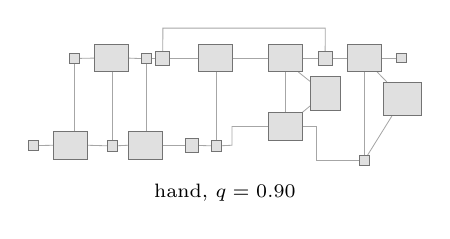
\begin{tikzpicture}[x=1cm,y=1cm,line width=0.3pt]
\draw[gray!70] (0.586,1.354) -- (0.842,1.359);
\draw[gray!70] (0.586,0.425) -- (0.586,1.354);
\draw[gray!70] (3.581,1.063) -- (3.429,1.185);
\draw[gray!70] (2.600,1.359) -- (3.056,1.359);
\draw[gray!70] (3.490,1.359) -- (3.772,1.359);
\draw[gray!70] (3.273,0.664) -- (3.273,1.185);
\draw[gray!70] (3.477,0.664) -- (3.581,0.751);
\draw[gray!70] (1.710,1.359) -- (2.166,1.359);
\draw[gray!70] (3.772,1.359) -- (3.774,1.740) -- (1.712,1.740) -- (1.710,1.359);
\draw[gray!70] (1.502,1.350) -- (1.710,1.359);
\draw[gray!70] (2.391,1.185) -- (2.391,0.243);
\draw[gray!70] (3.772,1.359) -- (4.054,1.359);
\draw[gray!70] (4.488,1.359) -- (4.744,1.359);
\draw[gray!70] (4.431,1.185) -- (4.557,1.055);
\draw[gray!70] (4.271,1.185) -- (4.271,0.061);
\draw[gray!70] (4.627,0.634) -- (4.271,0.061);
\draw[gray!70] (1.276,1.359) -- (1.502,1.350);
\draw[gray!70] (1.068,1.185) -- (1.068,0.243);
\draw[gray!70] (1.502,0.425) -- (1.502,1.350);
\draw[gray!70] (0.065,0.247) -- (0.321,0.252);
\draw[gray!70] (0.755,0.252) -- (1.068,0.243);
\draw[gray!70] (1.068,0.243) -- (1.276,0.252);
\draw[gray!70] (1.710,0.252) -- (2.079,0.252);
\draw[gray!70] (2.391,0.243) -- (2.589,0.252) -- (2.589,0.490) -- (3.056,0.490);
\draw[gray!70] (2.079,0.252) -- (2.391,0.243);
\draw[gray!70] (3.490,0.490) -- (3.659,0.490) -- (3.659,0.061) -- (4.271,0.061);
\draw[fill=black!12,draw=black!55] (0.521,1.289) rectangle (0.651,1.419);
\draw[fill=black!12,draw=black!55] (3.056,1.185) rectangle (3.490,1.532);
\draw[fill=black!12,draw=black!55] (3.581,0.699) rectangle (3.963,1.120);
\draw[fill=black!12,draw=black!55] (1.623,1.272) rectangle (1.797,1.445);
\draw[fill=black!12,draw=black!55] (2.166,1.185) rectangle (2.600,1.532);
\draw[fill=black!12,draw=black!55] (3.685,1.272) rectangle (3.859,1.445);
\draw[fill=black!12,draw=black!55] (4.054,1.185) rectangle (4.488,1.532);
\draw[fill=black!12,draw=black!55] (4.683,1.298) rectangle (4.805,1.419);
\draw[fill=black!12,draw=black!55] (4.514,0.634) rectangle (5.000,1.055);
\draw[fill=black!12,draw=black!55] (0.842,1.185) rectangle (1.276,1.532);
\draw[fill=black!12,draw=black!55] (1.437,1.285) rectangle (1.567,1.415);
\draw[fill=black!12,draw=black!55] (0.000,0.182) rectangle (0.130,0.312);
\draw[fill=black!12,draw=black!55] (0.321,0.078) rectangle (0.755,0.425);
\draw[fill=black!12,draw=black!55] (1.003,0.178) rectangle (1.133,0.308);
\draw[fill=black!12,draw=black!55] (1.276,0.078) rectangle (1.710,0.425);
\draw[fill=black!12,draw=black!55] (2.326,0.178) rectangle (2.457,0.308);
\draw[fill=black!12,draw=black!55] (3.056,0.317) rectangle (3.490,0.664);
\draw[fill=black!12,draw=black!55] (1.992,0.165) rectangle (2.166,0.339);
\draw[fill=black!12,draw=black!55] (4.210,0.000) rectangle (4.332,0.122);
\node[anchor=north,font=\scriptsize] at (2.50,-0.12) {hand, $q=0.90$};
\end{tikzpicture}
&
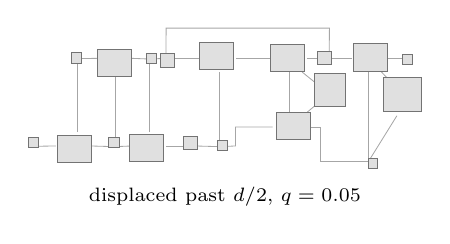
\begin{tikzpicture}[x=1cm,y=1cm,line width=0.3pt]
\draw[gray!70] (0.621,1.389) -- (0.878,1.393);
\draw[gray!70] (0.621,0.455) -- (0.621,1.389);
\draw[gray!70] (3.632,1.096) -- (3.480,1.219);
\draw[gray!70] (2.646,1.393) -- (3.104,1.393);
\draw[gray!70] (3.541,1.393) -- (3.824,1.393);
\draw[gray!70] (3.322,0.695) -- (3.322,1.219);
\draw[gray!70] (3.528,0.695) -- (3.632,0.782);
\draw[gray!70] (1.751,1.393) -- (2.209,1.393);
\draw[gray!70] (3.824,1.393) -- (3.827,1.777) -- (1.753,1.777) -- (1.751,1.393);
\draw[gray!70] (1.542,1.384) -- (1.751,1.393);
\draw[gray!70] (2.436,1.219) -- (2.436,0.271);
\draw[gray!70] (3.824,1.393) -- (4.108,1.393);
\draw[gray!70] (4.545,1.393) -- (4.802,1.393);
\draw[gray!70] (4.488,1.219) -- (4.614,1.088);
\draw[gray!70] (4.326,1.219) -- (4.326,0.088);
\draw[gray!70] (4.684,0.664) -- (4.326,0.088);
\draw[gray!70] (1.315,1.393) -- (1.542,1.384);
\draw[gray!70] (1.105,1.219) -- (1.105,0.271);
\draw[gray!70] (1.542,0.455) -- (1.542,1.384);
\draw[gray!70] (0.097,0.276) -- (0.354,0.280);
\draw[gray!70] (0.791,0.280) -- (1.105,0.271);
\draw[gray!70] (1.105,0.271) -- (1.315,0.280);
\draw[gray!70] (1.751,0.280) -- (2.122,0.280);
\draw[gray!70] (2.436,0.271) -- (2.635,0.280) -- (2.635,0.520) -- (3.104,0.520);
\draw[gray!70] (2.122,0.280) -- (2.436,0.271);
\draw[gray!70] (3.541,0.520) -- (3.711,0.520) -- (3.711,0.088) -- (4.326,0.088);
\draw[fill=black!12,draw=black!55] (0.546,1.332) rectangle (0.677,1.463);
\draw[fill=black!12,draw=black!55] (3.072,1.221) rectangle (3.509,1.570);
\draw[fill=black!12,draw=black!55] (3.642,0.782) rectangle (4.026,1.205);
\draw[fill=black!12,draw=black!55] (1.685,1.278) rectangle (1.859,1.453);
\draw[fill=black!12,draw=black!55] (2.170,1.251) rectangle (2.606,1.601);
\draw[fill=black!12,draw=black!55] (3.677,1.310) rectangle (3.851,1.484);
\draw[fill=black!12,draw=black!55] (4.131,1.230) rectangle (4.568,1.579);
\draw[fill=black!12,draw=black!55] (4.753,1.318) rectangle (4.875,1.440);
\draw[fill=black!12,draw=black!55] (4.511,0.723) rectangle (5.000,1.146);
\draw[fill=black!12,draw=black!55] (0.879,1.163) rectangle (1.316,1.512);
\draw[fill=black!12,draw=black!55] (1.503,1.326) rectangle (1.634,1.457);
\draw[fill=black!12,draw=black!55] (0.000,0.258) rectangle (0.131,0.389);
\draw[fill=black!12,draw=black!55] (0.374,0.071) rectangle (0.810,0.420);
\draw[fill=black!12,draw=black!55] (1.026,0.260) rectangle (1.157,0.391);
\draw[fill=black!12,draw=black!55] (1.286,0.078) rectangle (1.722,0.428);
\draw[fill=black!12,draw=black!55] (2.406,0.219) rectangle (2.537,0.350);
\draw[fill=black!12,draw=black!55] (3.155,0.360) rectangle (3.591,0.709);
\draw[fill=black!12,draw=black!55] (1.973,0.231) rectangle (2.147,0.406);
\draw[fill=black!12,draw=black!55] (4.316,0.000) rectangle (4.439,0.122);
\node[anchor=north,font=\scriptsize] at (2.50,-0.12) {displaced past $d/2$, $q=0.05$};
\end{tikzpicture}
&
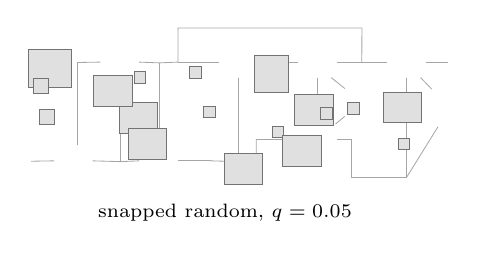
\begin{tikzpicture}[x=1cm,y=1cm,line width=0.3pt]
\draw[gray!70] (0.629,1.549) -- (0.919,1.554);
\draw[gray!70] (0.629,0.497) -- (0.629,1.549);
\draw[gray!70] (4.022,1.219) -- (3.850,1.357);
\draw[gray!70] (2.911,1.554) -- (3.427,1.554);
\draw[gray!70] (3.918,1.554) -- (4.238,1.554);
\draw[gray!70] (3.673,0.767) -- (3.673,1.357);
\draw[gray!70] (3.904,0.767) -- (4.022,0.865);
\draw[gray!70] (1.903,1.554) -- (2.419,1.554);
\draw[gray!70] (4.238,1.554) -- (4.240,1.986) -- (1.905,1.986) -- (1.903,1.554);
\draw[gray!70] (1.667,1.544) -- (1.903,1.554);
\draw[gray!70] (2.675,1.357) -- (2.675,0.290);
\draw[gray!70] (4.238,1.554) -- (4.558,1.554);
\draw[gray!70] (5.049,1.554) -- (5.339,1.554);
\draw[gray!70] (4.985,1.357) -- (5.128,1.209);
\draw[gray!70] (4.803,1.357) -- (4.803,0.084);
\draw[gray!70] (5.206,0.733) -- (4.803,0.084);
\draw[gray!70] (1.411,1.554) -- (1.667,1.544);
\draw[gray!70] (1.175,1.357) -- (1.175,0.290);
\draw[gray!70] (1.667,0.497) -- (1.667,1.544);
\draw[gray!70] (0.039,0.295) -- (0.329,0.300);
\draw[gray!70] (0.821,0.300) -- (1.175,0.290);
\draw[gray!70] (1.175,0.290) -- (1.411,0.300);
\draw[gray!70] (1.903,0.300) -- (2.321,0.300);
\draw[gray!70] (2.675,0.290) -- (2.898,0.300) -- (2.898,0.570) -- (3.427,0.570);
\draw[gray!70] (2.321,0.300) -- (2.675,0.290);
\draw[gray!70] (3.918,0.570) -- (4.110,0.570) -- (4.110,0.084) -- (4.803,0.084);
\draw[fill=black!12,draw=black!55] (2.232,0.846) rectangle (2.380,0.993);
\draw[fill=black!12,draw=black!55] (1.155,0.649) rectangle (1.647,1.042);
\draw[fill=black!12,draw=black!55] (2.871,1.163) rectangle (3.304,1.640);
\draw[fill=black!12,draw=black!55] (3.441,0.413) rectangle (3.638,0.610);
\draw[fill=black!12,draw=black!55] (0.831,0.993) rectangle (1.323,1.386);
\draw[fill=black!12,draw=black!55] (0.143,0.762) rectangle (0.339,0.959);
\draw[fill=black!12,draw=black!55] (3.382,0.752) rectangle (3.874,1.146);
\draw[fill=black!12,draw=black!55] (3.102,0.595) rectangle (3.240,0.733);
\draw[fill=black!12,draw=black!55] (0.000,1.236) rectangle (0.551,1.713);
\draw[fill=black!12,draw=black!55] (2.488,0.000) rectangle (2.979,0.393);
\draw[fill=black!12,draw=black!55] (3.717,0.826) rectangle (3.864,0.973);
\draw[fill=black!12,draw=black!55] (1.347,1.288) rectangle (1.495,1.436);
\draw[fill=black!12,draw=black!55] (3.230,0.231) rectangle (3.722,0.624);
\draw[fill=black!12,draw=black!55] (2.055,1.352) rectangle (2.203,1.500);
\draw[fill=black!12,draw=black!55] (1.268,0.320) rectangle (1.760,0.713);
\draw[fill=black!12,draw=black!55] (4.061,0.890) rectangle (4.208,1.037);
\draw[fill=black!12,draw=black!55] (4.508,0.782) rectangle (5.000,1.175);
\draw[fill=black!12,draw=black!55] (0.064,1.155) rectangle (0.261,1.352);
\draw[fill=black!12,draw=black!55] (4.700,0.447) rectangle (4.838,0.585);
\node[anchor=north,font=\scriptsize] at (2.50,-0.12) {snapped random, $q=0.05$};
\end{tikzpicture}
\end{tabular}
\caption{The alignment controls on one BPMN model (19 boxes; the corpus medians are
$0.91$, $0.20$ and $0.07$). Left, the drawing as its author left it. Centre, every box
displaced by up to 15 units, just past the $d/2$ below which the directional test cannot
resolve a misalignment. Right, every box placed uniformly at random in the same bounding
box and snapped to the same grid: the grid is available and the author is not. Box sizes
are unchanged throughout; edges are the routes the file stores.}
\label{fig:controls}
\end{figure}


\paragraph{The editor snapped to a grid,} so alignment is the tool's. Excluded. The
detected pitch is one unit in Reactome and BPMN (67\% and 63\% integer coordinates) and
none in WikiPathways (17\%, against 0.37 of boxes exactly aligned in $x$). A layout
snapped to the same grid, with the same boxes and the same bounding box and no author,
holds 0.065, 0.075 and 0.067 (Figure~\ref{fig:controls}); snapped to the plausible
working pitch of five units, 0.076. The grid is available to the random layout and does
not produce the effect. Displacing every hand-placed box by up to half a pitch leaves the
hold where it was, and that test cannot fail, for a reason in the instrument: a box
offset by $\epsilon$ from its nearest agreement is released only by a move whose
component toward the agreement, $a$, exceeds $2\epsilon$; the smallest such component
among sixteen directions is $0.38\,d$, so release begins at $\epsilon > 0.19\,d$, which is
3 to 5 units against a half pitch of 0.5. Displacing past that takes the hand layouts to
the snapped random level (0.065 to 0.062 at a half-width of 120 units;
Appendix~\ref{app:corpus}).

\paragraph{The editor snapped to the neighbours,} so alignment is the guide's. Not
separable on these corpora, and conceded. A grid control cannot see snap-to-object
guides, which PathVisio and the BPMN editors draw on every drag and Reactome's curation
tool does not, and the alignment hold orders as those affordances do: 0.85 where guides
meet every drag, 0.52 where they are offered, 0.21 where they are absent. Two pieces of
evidence say no single editor's aid produces the hold. HOLA's drawings come from a study
tool, not a commercial editor, and hold 0.50. The GD Collection by era holds 0.81 in
1998 to 2005, when its figures came from xfig, Ipe and hand-coded PostScript with no
shared guide, 0.60 in 2006 to 2014 and 0.95 in the TikZ years, where a typed coordinate is
alignment chosen by hand; and WikiPathways is flat at 0.47 to 0.53 across four
generations of pathway numbers, so no gradient follows PathVisio's releases
(\texttt{results/era.md}). What stays open is whether some aid does in each era.
Separating hand from guide needs a guide-free editor or an interaction log, and these
corpora carry neither. Marriott et al.\ \cite{marriott12} bound the other side: in a
recall task node alignment was the one feature participants did not preserve while
orthogonality, collinearity and symmetry were, so the alignment these coordinates hold is
a property of how the layouts were made, not evidence that anyone perceived it. Every
claim here is about the coordinates as data for a fit, and for a fit the attribution
changes nothing: the coordinates hold a term the energy lacks either way.

\paragraph{The lanes hold the boxes.} 82\% of BPMN boxes sit in a lane or pool, and a
horizontal lane constrains $y$. Per held box, the alignment that holds it: 28\% a column,
which no horizontal lane imposes; 14\% a row shared with a box of another lane or of no
lane; 58\% a row within one lane, and those lanes are a median 6.3 box heights tall
(quartiles 3.7 and 9.4), so the row inside them was chosen (\texttt{results/lanes.py}).

The rest, each with the test that excluded it:

\begin{center}\small
\begin{tabular}{@{}>{\raggedright\arraybackslash}p{2.6cm}>{\raggedright\arraybackslash}p{4.2cm}>{\raggedright\arraybackslash}p{7.5cm}@{}}
\toprule
alternative & test & result \\
\midrule
Reference length & $L$ at the median edge length and at $1/\sqrt{N}$ & hand held on 0.00 to 0.05 of boxes under length and stress; only the control moves (Appendix~\ref{app:reference}) \\[2pt]
Centre distances on box diagrams & border-to-border distances, $L$ refitted & hand 0.00 in every corpus; \texttt{neato}, which minimised the centre form, not held under the border form \\[2pt]
Straight segments where the person drew polylines & the tables on the stored routes, chords beside them & no verdict moves \\[2pt]
The radius and the directions & $d \in \{0.005, 0.01, 0.02, 0.05\}$; 8 to 64 directions & hand verdicts the same at every $d$ and count; the A1 level falls with the direction count (0.52 to 0.39 on WikiPathways at 64), the gap to the control does not (Appendix~\ref{app:radius}) \\[2pt]
Near-trees make overlap and crossings easy & $q$ against $m/n$ over diagrams & crossings track density (Spearman $-0.11$ to $-0.37$) for hand and tool alike; length and stress are 0.00 in the sparse and the dense half both \\[2pt]
Reading direction is the missing constraint & the flow term & flow holds 0.59 to 0.86 of hand-placed boxes where \texttt{dot} and ELK hold 1.00: a criterion partly satisfied, the person tolerating a backward edge \\[2pt]
The tools are the wrong tools & ELK layered, the engine the BPMN editors run & its profile is \texttt{dot}'s: distance terms 0.00, flow 1.00, alignment 0.42 to 0.59 \\
\bottomrule
\end{tabular}
\end{center}

\section{Related work}\label{sec:related}

Aesthetic criteria and their weighting go back to Tamassia, Di Battista and Batini
\cite{tdb88} and were made an explicit energy by Davidson and Harel \cite{dh96}. Purchase
\cite{purchase02} gave the criteria their metrics, among them node orthogonality, the fit
of node positions to an imaginary grid; Bennett et al.'s survey \cite{bennett07} lists it
and uniform edge length side by side, each with a Gestalt rationale and, as of 2007,
neither evaluated. The test here is such an evaluation, at the coordinates, and it
separates the two.

\begin{center}\small
\begin{tabular}{@{}>{\raggedright\arraybackslash}p{3.4cm}>{\raggedright\arraybackslash}p{5.2cm}>{\raggedright\arraybackslash}p{5.7cm}@{}}
\toprule
work & what it did & what it gives, and what it leaves \\
\midrule
\multicolumn{3}{@{}l}{\emph{By having people draw}}\\[2pt]
van Ham, Rogowitz \cite{vanham08} & 73 hand layouts against a force-directed algorithm, half started from its optimum & 71 of 73 raise edge-length variance above the optimum; a value, not a test \\[2pt]
Dwyer et al.\ \cite{dwyer09} & 32 participants laid out one graph; 194 judges ranked the results & judges' choices track stress; the user layouts carry 3 to 9 times the force-directed stress in that paper's Table 2 \\[2pt]
Purchase, Pilcher, Plimmer \cite{purchase12} & participants drew from adjacency lists & crossing removal the strongest aesthetic, alignment to a grid important \\[2pt]
Kieffer et al.\ \cite{hola16} & 17 participants' layouts of 8 graphs, ranked by 66 judges & gridiness correlates with rank on all 8, the source of HOLA's alignment step \\[2pt]
Marriott et al.\ \cite{marriott12} & 25 participants redrew small diagrams from memory & symmetry, collinearity and orthogonality preserved; node alignment not \\[2pt]
Mooney et al.\ \cite{mooney25, gdcoll25} & preference and performance against stress; 4,890 drawings harvested from these proceedings & people prefer low stress and perform better as it falls; the collection is measured in Section~\ref{sec:results} \\[4pt]
\multicolumn{3}{@{}l}{\emph{By learning from examples}}\\[2pt]
Masui \cite{masui94}; Sp\"onemann et al.\ \cite{spoenemann14}; Klammler et al.\ \cite{klammler19}; Zhang et al.\ \cite{zhang26} & weights from good and bad layouts, from selections, from good-against-worsened pairs, from 64,222 preference labels & none tests whether an example is a minimum of the learned energy; none fits coordinates \\[2pt]
Flud \cite{flud22} & annealing continued from crowd layouts of pathway diagrams & the closest prior descent from a hand layout; a rising asserted score read as success, without a cap, a reference or a per-term reading \\[2pt]
O'Donovan, Agarwala, Hertzmann \cite{odonovan14} & a 122-parameter energy over single-page designs fitted by inverse optimisation & each example taken as optimal: the assumption examined here; their term set contains alignment \\
\bottomrule
\end{tabular}
\end{center}

Alignment as a human criterion is known since 2012 in graph drawing and since 1985 in
drawing editors: Pavlidis and Van Wyk's beautifier inferred alignment constraints from the
near-alignments of a rough drawing \cite{pvw85}, Igarashi et al.\ made the inference
interactive \cite{igarashi97}, and the guides of Section~\ref{sec:alternatives} are their
descendants. The new part is the count of how many hand-placed boxes it holds beside the
counts for the criteria tools weight, and the step under the distance terms. Van
Wageningen, Mchedlidze and Telea \cite{wageningen25} show drawings with identical metric
values that differ in quality, so a fitted energy with no residual would still not be the
energy people use; the claims here stay on the negative side.

The machinery is standard elsewhere. Inverse optimisation is due to Ahuja and Orlin
\cite{ahuja01} for linear programs and to Keshavarz, Wang and Boyd \cite{keshavarz11} for
the convex case, whose first-order residual is the one reported here; Chan, Lee and
Terekhov \cite{chan19} give its geometry. The degenerate vertex is Ng and Russell's
\cite{ng00}, the margin repair Ratliff, Bagnell and Zinkevich's \cite{ratliff06}, and the
premise that demonstrations are only near-optimal is where learning from demonstration
went in 2008 \cite{ziebart08} and inverse optimisation in 2018 \cite{aswani18}; the
graph-drawing proposal predates that turn and a coordinate fit to the new corpus would
rest on the older premise. Matched-budget random controls are standard in hyperparameter
search \cite{bergstra12} and were prescribed for genetic algorithms in 1995 \cite{jw95};
Marriott et al.'s test of feature preservation against random redrawings
\cite{marriott12} is the nearest precedent in layout to the nulls used here.

\section{What follows}\label{sec:discussion}

Coordinates a person accepted are not minima of the energy in use. The failure is the
assumption's, not the drawing's, and it is specific: overlap is met exactly, uniform edge
length and stress are nowhere near met, and what holds the boxes instead is an alignment
into rows and columns that, HOLA's gridiness step aside \cite{hola16}, no force-directed
or multicriteria energy prices. The charge is bounded: \texttt{dot} and ELK hold alignment
at 0.42 to 1.00 without pricing it, since layering aligns as a side effect, so the missing
term convicts the energies, not the layered engines.

\paragraph{For a tool that learns its weights.} Offer alignment among the terms or the
fit returns nothing the drawing did. That is one addition, not a subtraction: edge length
and stress keep their weight, since a term inert at human coordinates is not thereby
unwanted, and the preference evidence runs the other way \cite{mooney25, dwyer09}. People
prefer the layouts a stress minimiser makes, do not draw that way, and do not notice the
alignment they do draw \cite{marriott12}; production and perception are measured on
different graphs and tasks, and no study yet takes both from one corpus. The number to
report for a fitted energy is the fraction of a held-out drawing's boxes it holds,
$q_{0.02}$ at sixteen directions with the fitted $L$, with the decrease and active columns
beside it, since a bare held fraction can always be bought by weighting a term everyone
satisfies. The size of the gain is measured: deleting each box in turn and letting the
energy replace it against the frozen rest, alignment does not move the median distance to
the person's position (the distance terms choose the neighbourhood) and raises the share
of boxes landing within 0.005 of the person's row or column from 0.085, 0.083 and 0.162 to
0.127, 0.101 and 0.226, chance 0.02, every diagram-clustered interval excluding zero
(Appendix~\ref{app:reinsert}).

\paragraph{Where the test applies.} The test is a diagnostic to run before fitting any
decomposable objective to artefacts taken as optimal, wherever the analyst can move one
variable at a time: page and interface layout \cite{odonovan14}, label placement,
floorplans, sketch beautification, and learning from demonstration under a static cost.
It sorts the terms into three classes before any weight is fitted: satisfied (held at
value zero, the source of the trivial solution), inert (flat at the demonstration radius,
held without being met, the active column), and violated (an improving move at almost
every demonstration, so no positive weight is feasible). A candidate term that holds a
large fraction of the demonstrations while the fitted energy holds none is a missing
feature, found without fitting. Two things do not transfer: the condition for a
sequential decision is optimality along a trajectory, not stationarity of an endpoint;
and a contrastive fit, which reads a weight off the gap between the demonstration and its
alternatives, can put weight on a term the coordinate fit cannot, since hand layouts
carry far less stress than random ones.

\paragraph{Limits.} The alignment count is specific to box-and-arrow diagrams of 4 to 100
boxes drawn in editors with guides, and it falls with size. The hand is not separated from
the guide. The GD Collection is measured on chord edges with no box sizes, so its profile
is on three terms. The BPMN corpus is a sample of 300 from 6,723; the alignment hold over
the population is 0.87. The first-order residual is a scale-dependent number and is
reported only beside $q$.

\section{Reproducibility}\label{sec:repro}

Parsers, the energy (one function per term), the directional test, the descent, the
fitting scripts, the parsed corpora and every table's script are in the repository under
\texttt{example/diagrams}. The directional test is deterministic; the descents are
deterministic from their seed on every platform. The main tables rebuild by
\texttt{results/run\_all.sh} and \texttt{profile.py --corpora BPMN:bpmnr}, the paired tests by
\texttt{results/tests.sh}, and the nulls, the alignment controls, the HOLA and GD
Collection runs, the era, dedup and drawer analyses, the calibration and the reinsertion
each ship their script beside their committed output. \texttt{results/manifest.txt}
records the commit, the platform, the tool versions (gcc 13.3.0, Graphviz 2.43.0, elkjs
0.12.0, HiGHS via scipy 1.18.1), the seeds and the SHA-256 of the three raw archives and
of the corpus files as measured. The BPMN archive is distributed for academic use; the
repository carries only derived coordinates and ids, never model content, and the two
biological corpora are CC-licensed exports. The plan the study was run to, signed on
22 August 2026, is beside the paper as \texttt{PREREGISTRATION-STATIONARITY.md}; its
hypotheses and their outcomes are in Appendix~\ref{app:plan}.

\appendix

\section{The summed energies, \texttt{prism} and the smooth kernel}\label{app:sums}

$q_{0.02}$ under the summed energies at equal weights, and the two columns the main
table omits.

\begin{center}\scriptsize\setlength{\tabcolsep}{3.5pt}
\begin{tabular}{llrrrrr}
\toprule
corpus & energy & hand & \texttt{neato} & \texttt{prism} & \texttt{dot} & ELK \\
\midrule
WikiPathways & alignment A3 alone & 0.20 [0.18, 0.23] (0.284) & 0.03 (0.446) & 0.03 (0.451) & 0.45 (0.204) & 0.35 (0.176) \\
& overlap alone, \texttt{prism} & & & 1.00 (0.000) & & \\
& length alone, \texttt{prism} & & & 0.19 (0.014) & & \\
& stress alone, \texttt{prism} & & & 0.94 (0.044) & & \\
& C$+$O & 1.00 [1.00, 1.00] & 0.60 & 1.00 & 1.00 & 1.00 \\
& C$+$O$+$L & 0.00 [0.00, 0.00] & 0.17 & 0.19 & 0.00 & 0.00 \\
& C$+$O$+$S & 0.00 [0.00, 0.00] & 0.60 & 0.94 & 0.00 & 0.00 \\
& C$+$O$+$R & 0.21 [0.19, 0.23] & 0.00 & 0.00 & 0.19 & 0.22 \\
& C$+$O$+$A1 & 0.51 [0.47, 0.53] & 0.04 & 0.07 & 1.00 & 0.57 \\
& C$+$O$+$A3 & 0.24 [0.22, 0.27] & 0.03 & 0.03 & 0.50 & 0.41 \\
& C$+$O$+$grid & 0.84 [0.81, 0.87] & 0.45 & 0.79 & 0.96 & 0.74 \\
& C$+$O$+$N & 0.86 [0.83, 0.88] & 0.55 & 1.00 & 0.78 & 0.74 \\
& C$+$O$+$F & 0.56 [0.53, 0.59] & 0.30 & 0.50 & 1.00 & 1.00 \\
\midrule
Reactome & alignment A3 alone & 0.10 [0.08, 0.12] (0.300) & 0.03 (0.430) & 0.03 (0.428) & 0.39 (0.206) & 0.31 (0.213) \\
& overlap alone, \texttt{prism} & & & 1.00 (0.000) & & \\
& length alone, \texttt{prism} & & & 0.26 (0.009) & & \\
& stress alone, \texttt{prism} & & & 0.85 (0.042) & & \\
& C$+$O & 1.00 [1.00, 1.00] & 0.76 & 1.00 & 1.00 & 1.00 \\
& C$+$O$+$L & 0.00 [0.00, 0.00] & 0.33 & 0.27 & 0.00 & 0.00 \\
& C$+$O$+$S & 0.00 [0.00, 0.00] & 0.76 & 0.89 & 0.00 & 0.00 \\
& C$+$O$+$R & 0.17 [0.16, 0.19] & 0.00 & 0.00 & 0.14 & 0.13 \\
& C$+$O$+$A1 & 0.22 [0.19, 0.25] & 0.05 & 0.07 & 1.00 & 0.43 \\
& C$+$O$+$A3 & 0.11 [0.09, 0.12] & 0.03 & 0.03 & 0.42 & 0.33 \\
& C$+$O$+$grid & 0.64 [0.61, 0.67] & 0.52 & 0.75 & 0.94 & 0.73 \\
& C$+$O$+$N & 0.94 [0.91, 0.95] & 0.71 & 1.00 & 0.80 & 0.75 \\
& C$+$O$+$F & 0.61 [0.58, 0.65] & 0.33 & 0.44 & 1.00 & 1.00 \\
\midrule
BPMN & alignment A3 alone & 0.33 [0.28, 0.35] (0.213) & 0.00 (0.454) & 0.00 (0.453) & 0.21 (0.187) & 0.22 (0.163) \\
& overlap alone, \texttt{prism} & & & 1.00 (0.000) & & \\
& length alone, \texttt{prism} & & & 0.26 (0.011) & & \\
& stress alone, \texttt{prism} & & & 0.93 (0.022) & & \\
& C$+$O & 1.00 [1.00, 1.00] & 0.41 & 1.00 & 1.00 & 1.00 \\
& C$+$O$+$L & 0.00 [0.00, 0.00] & 0.21 & 0.28 & 0.00 & 0.00 \\
& C$+$O$+$S & 0.00 [0.00, 0.00] & 0.44 & 0.93 & 0.00 & 0.00 \\
& C$+$O$+$R & 0.74 [0.71, 0.76] & 0.00 & 0.00 & 0.29 & 0.39 \\
& C$+$O$+$A1 & 0.85 [0.82, 0.89] & 0.04 & 0.09 & 0.95 & 0.67 \\
& C$+$O$+$A3 & 0.35 [0.31, 0.38] & 0.03 & 0.03 & 0.33 & 0.41 \\
& C$+$O$+$grid & 0.94 [0.93, 0.95] & 0.30 & 0.78 & 0.81 & 0.66 \\
& C$+$O$+$N & 1.00 [1.00, 1.00] & 0.40 & 1.00 & 0.86 & 0.79 \\
& C$+$O$+$F & 0.86 [0.82, 0.88] & 0.25 & 0.61 & 1.00 & 1.00 \\
\bottomrule
\end{tabular}
\end{center}

At the hand layout the three base terms share the energy as length 0.99, crossings 0.01,
overlap 0.00, and $C{+}O{+}L$ inherits the length term's zero.

\section{Radius and directions}\label{app:radius}

$q_d$ at $d \in \{0.005, 0.01, 0.02, 0.05\}$, hand layouts and \texttt{neato}'s
(\texttt{profile.py --sweep}; BPMN on the first-300 sample).

\begin{center}\footnotesize
\begin{tabular}{lrrrrrrrrrrrr}
\toprule
 & \multicolumn{4}{c}{WikiPathways} & \multicolumn{4}{c}{Reactome} & \multicolumn{4}{c}{BPMN} \\
energy & .005 & .01 & .02 & .05 & .005 & .01 & .02 & .05 & .005 & .01 & .02 & .05 \\
\midrule
overlap, hand & 1.00 & 1.00 & 1.00 & 1.00 & 1.00 & 1.00 & 1.00 & 1.00 & 1.00 & 1.00 & 1.00 & 1.00 \\
length, hand & 0.00 & 0.00 & 0.00 & 0.00 & 0.00 & 0.00 & 0.00 & 0.00 & 0.00 & 0.00 & 0.00 & 0.00 \\
stress, hand & 0.00 & 0.00 & 0.00 & 0.00 & 0.00 & 0.00 & 0.00 & 0.00 & 0.00 & 0.00 & 0.00 & 0.00 \\
alignment A1, hand & 0.52 & 0.54 & 0.52 & 0.44 & 0.12 & 0.17 & 0.21 & 0.19 & 0.90 & 0.91 & 0.91 & 0.87 \\
gridiness, hand & 0.94 & 0.91 & 0.87 & 0.75 & 0.82 & 0.75 & 0.65 & 0.57 & 1.00 & 1.00 & 0.95 & 0.88 \\
flow, hand & 0.59 & 0.59 & 0.59 & 0.59 & 0.62 & 0.62 & 0.62 & 0.63 & 0.85 & 0.85 & 0.85 & 0.85 \\
\midrule
length, \texttt{neato} & 0.04 & 0.12 & 0.24 & 0.47 & 0.07 & 0.19 & 0.35 & 0.58 & 0.08 & 0.22 & 0.42 & 0.72 \\
stress, \texttt{neato} & 0.90 & 0.96 & 1.00 & 1.00 & 0.96 & 1.00 & 1.00 & 1.00 & 0.94 & 0.97 & 1.00 & 1.00 \\
alignment A1, \texttt{neato} & 0.04 & 0.05 & 0.06 & 0.06 & 0.03 & 0.05 & 0.06 & 0.07 & 0.03 & 0.05 & 0.06 & 0.07 \\
\bottomrule
\end{tabular}
\end{center}

The hand verdicts do not move with the radius. \texttt{neato}'s under length do: a layout
that is nearly a minimum is held at a large radius and free at a small one, and
\texttt{neato}'s layouts, which minimise stress and not length uniformity, read as nearly
uniform at $d = 0.05$ and not at $d = 0.005$. A hand layout at 0.00 across the range is
far from the minimum at every scale the test resolves. At $d$ equal to one grid pitch,
0.0008 to 0.0017 of the width, hand length and stress still hold 0.00
(\texttt{results/pitch.md}).

Each doubling of $V$ contains the previous set, so $q$ can only fall as directions are
added and the sixteen-direction figures are upper bounds on the continuum value. At 8, 16,
32 and 64 directions hand length and stress read 0.00 and \texttt{neato}'s stress 1.00 in
every corpus. The A1 level falls: 0.58, 0.52, 0.47, 0.39 on WikiPathways, 0.31, 0.21,
0.14, 0.07 on Reactome, 0.92, 0.91, 0.90, 0.86 on BPMN, while \texttt{neato}'s 0.06 falls
to 0.00. This is the corner's release bound of Section~\ref{sec:alternatives} at work, and
at the continuum limit the hold is the exact-tie fraction. The gap survives at 64; levels
are stated at sixteen. The full grid of radius, direction count, reference-length rule and
route treatment, 1,008 cells, flips no verdict (\texttt{results/specgrid.md}); the tie
tolerance moves nothing between 0.001 and 0.01 (\texttt{results/tolsweep.md}).

\section{Reference length and box extent}\label{app:reference}

Under the median edge length instead of the fitted $L$, \texttt{neato}'s stress layouts
score 0.07, 0.08 and 0.12 under stress and the hand layouts 0.00; under length the hand
layouts score 0.03, 0.04 and 0.05 and \texttt{neato}'s 0.26, 0.41 and 0.45. Under
$L = 1/\sqrt{N}$ no box of any layout is held under either term. The fitted $L$ is the
only rule under which a true minimum of the term is a fixed point of the test, and the
hand verdicts are 0.00 to 0.05 under every rule.

Measured border to border, each box's offset to its border along the joining direction
subtracted and $L$ refitted on those distances, length and stress hold 0.00 of the hand
layouts in every corpus, 0.86 to 0.92 of diagrams at exactly zero
(\texttt{results/border.py}); \texttt{neato}, which minimised the centre form, is not held
under the border form (0.00 to 0.09).

\section{Descent, chance and calibration}\label{app:descent}

The secondary estimand: hill climbing from the hand layout, each proposal one box moved a
random step, kept when the energy falls, every box confined to a circle of radius 0.02
about its start, 15 seeds, against uniform sampling in the same circles at the same
budget. Per corpus and energy: the median fraction of the cap the climber uses and of the
energy it removes, the same for the sampler, the share of diagrams where the climber ends
lower on at least 12 of 15 seeds, and $q_{0.02}$ where the uncapped climber stops, the
converged reference. BPMN on the first-300 sample.

\begin{center}\footnotesize
\begin{tabular}{llrrrrrr}
\toprule
 & & \multicolumn{2}{c}{cap used} & \multicolumn{2}{c}{energy removed} & & \\
corpus & energy & climb & random & climb & random & $\ge$12/15 & $q$ conv. \\
\midrule
WikiPathways & C$+$O$+$L & 0.99 & 0.76 & 0.28 & 0.16 & 0.88 & 1.00 \\
 & C$+$O$+$A1 & 0.39 & 0.74 & 0.71 & 0.17 & 0.75 & 1.00 \\
 & stress & 1.00 & 0.77 & 0.12 & 0.05 & 1.00 & 1.00 \\
 & C$+$O$+$F & 0.44 & 0.76 & 0.27 & 0.18 & 0.77 & 1.00 \\
\midrule
Reactome & C$+$O$+$L & 1.00 & 0.76 & 0.31 & 0.16 & 0.93 & 1.00 \\
 & C$+$O$+$A1 & 0.56 & 0.74 & 0.99 & 0.37 & 0.80 & 1.00 \\
 & stress & 1.00 & 0.77 & 0.13 & 0.06 & 1.00 & 1.00 \\
 & C$+$O$+$F & 0.36 & 0.75 & 0.32 & 0.22 & 0.71 & 1.00 \\
\midrule
BPMN & C$+$O$+$L & 1.00 & 0.77 & 0.26 & 0.12 & 0.99 & 1.00 \\
 & C$+$O$+$A1 & 0.11 & 0.73 & 0.24 & $-$0.01 & 0.95 & 1.00 \\
 & stress & 1.00 & 0.77 & 0.14 & 0.07 & 1.00 & 1.00 \\
 & C$+$O$+$F & 0.16 & 0.74 & 0.09 & 0.04 & 0.66 & 1.00 \\
\bottomrule
\end{tabular}
\end{center}

Under the distance energies the climber walks every box to the cap circle and is still
removing energy when the budget ends; under C$+$O$+$A1 it moves 0.11 to 0.56 of the cap,
the misalignments being nearer than $d$. The converged reference's median $q$ is 1.00 for
every energy and corpus; the fraction of diagrams whose reference stops below 0.9 is at
most 0.02 everywhere but C$+$O$+$F (0.05 to 0.13), the flow term's plateaus.

Calibration (\texttt{results/calib.py}): the median fraction of the stress energy the
same capped climber removes from \texttt{neato}'s converged layouts after every box is
displaced by $\epsilon$ of the width in a seeded direction.

\begin{center}\footnotesize
\begin{tabular}{lrrrrrr}
\toprule
$\epsilon$ & 0 & 0.005 & 0.01 & 0.02 & 0.05 & hand layouts \\
\midrule
WikiPathways & 0.001 & 0.007 & 0.024 & 0.087 & 0.245 & 0.116 \\
Reactome & 0.001 & 0.009 & 0.033 & 0.116 & 0.289 & 0.128 \\
BPMN & 0.001 & 0.024 & 0.084 & 0.261 & 0.427 & 0.145 \\
\bottomrule
\end{tabular}
\end{center}

\section{The paired tests}\label{app:paired}

Per corpus, hand against \texttt{dot} on each criterion alone: the Hodges--Lehmann shift
of $q_{0.02}$ with its 95\% interval, zeros dropped, and the Holm-adjusted signed-rank $p$
within the corpus's family (\texttt{analyse.py}, 630 self-checks against enumeration and
against R; the families against \texttt{neato}, \texttt{prism} and ELK in
\texttt{results/tests/}). WikiPathways and Reactome as measured; BPMN on the first-300
sample except the alignment row, which is the random 300.

\begin{center}\scriptsize
\begin{tabular}{lrrrrrr}
\toprule
 & \multicolumn{2}{c}{WikiPathways} & \multicolumn{2}{c}{Reactome} & \multicolumn{2}{c}{BPMN} \\
energy & HL [95\%] & $p$ & HL [95\%] & $p$ & HL [95\%] & $p$ \\
\midrule
crossings & $-0.04$ [$-0.07$, $-0.01$] & 0.016 & $+0.02$ [$-0.01$, $+0.05$] & 0.30 & $+0.10$ [$+0.08$, $+0.12$] & $<$1e-4 \\
overlap & $-0.14$ [$-0.18$, $-0.11$] & $<$1e-4 & $-0.07$ [$-0.10$, $-0.06$] & 0.0024 & $-0.22$ [$-0.29$, $-0.11$] & $<$1e-4 \\
length & $-0.01$ [$-0.03$, $+0.00$] & 0.27 & $-0.03$ [$-0.05$, $-0.01$] & 0.017 & $-0.09$ [$-0.12$, $-0.06$] & $<$1e-4 \\
stress & $-0.03$ [$-0.04$, $-0.00$] & 0.022 & $-0.03$ [$-0.05$, $-0.01$] & 0.0048 & $-0.08$ [$-0.11$, $-0.05$] & $<$1e-4 \\
orthogonality & $+0.01$ [$-0.00$, $+0.04$] & 0.27 & $+0.02$ [$+0.00$, $+0.04$] & 0.036 & $+0.43$ [$+0.41$, $+0.45$] & $<$1e-4 \\
alignment A1 & $-0.46$ [$-0.49$, $-0.43$] & $<$1e-4 & $-0.70$ [$-0.73$, $-0.67$] & $<$1e-4 & $-0.05$ [$-0.10$, $-0.00$] & 0.042 \\
node--edge & $+0.13$ [$+0.10$, $+0.16$] & $<$1e-4 & $+0.18$ [$+0.15$, $+0.21$] & $<$1e-4 & $+0.26$ [$+0.23$, $+0.28$] & $<$1e-4 \\
flow & $-0.40$ [$-0.42$, $-0.38$] & $<$1e-4 & $-0.33$ [$-0.35$, $-0.31$] & $<$1e-4 & $-0.17$ [$-0.19$, $-0.14$] & $<$1e-4 \\
\bottomrule
\end{tabular}
\end{center}

The shifts under crossings, overlap, length and stress are confined to the minority of
diagrams where the pair differs at all. The large shifts are the profile's gaps: the hand
layout sits below \texttt{dot} on alignment in every corpus, below it on flow, and above it
on node--edge separation and, in BPMN, on orthogonality, the criteria \texttt{dot} trades
away.

\section{The BPMN samples}\label{app:bpmn}

The study was planned on the first 300 models by id. On all 6,723 models in the band
the alignment hold is 0.87 (mean 0.81; \texttt{data/bpmn\_population\_a1.csv},
regenerated from the archive by the commands in its header), against 0.91 on the first
300, which resampling 300 of the population 2,000 times puts at the 99th percentile,
outside the interval [0.83, 0.90] a random 300 gives. Every other term is where it was:
crossings, overlap and node--edge at 1.00, length and stress at 0.00, orthogonality 0.733
against 0.726, flow 0.842 against 0.854 (\texttt{results/bpmn\_population.md}). The
seeded random 300 (\texttt{random.Random(1)}, \texttt{data/bpmnr.txt}) with all four tool
controls regenerated is the corpus of the main tables; its A1 hold is 0.85 (0.846), every
other energy within 0.017 of the first 300, and the one paired verdict that changes is
hand against \texttt{dot} on alignment, parity on the first 300 (HL $+0.04$
[$-0.01$, $+0.09$]) and below on the random 300 ($-0.05$ [$-0.10$, $-0.00$], Holm
$p = 0.042$), as in the other corpora (\texttt{results/bpmn\_random300.md}). The analyses
this appendix marks as on the first 300 predate the switch and were not rerun; none of
them carries an alignment level in the main text.

\section{Corpus checks}\label{app:corpus}

\paragraph{Deduplication} (\texttt{results/dedup.py}): by exact coordinate multiset, one
Reactome pair is a single drawing stored under two ids; by the structural key ($n$, $m$,
degree sequence, box sizes), one further Reactome pair and one WikiPathways pair; the BPMN
models collide under neither key. Removing every extra member moves no headline median.

\paragraph{Drawers} (\texttt{results/drawers.py}): the 305 WikiPathways pathways carry
153 first authors, the most prolific 9\% of the corpus; the A1 median's interval clustered
by first author is [0.48, 0.55] against [0.48, 0.54] over diagrams, and the twenty drawers
of three or more pathways hold medians 0.19 to 0.85. Reactome curators and BPMN authors
are not recorded in the archives as parsed.

\paragraph{The 41 to 100 band} (\texttt{results/band41.md}; 108, 265 and 300 diagrams,
against \texttt{neato}): length and stress hold 0.00 by hand in every corpus and
\texttt{neato}'s stress 1.00; overlap 1.00; alignment 0.39, 0.16 and 0.74 against
\texttt{neato}'s 0.07 to 0.08. Larger diagrams carry less alignment, and crossings stop
holding every biological box (0.97 and 0.98).

\paragraph{The grid controls} (\texttt{results/align\_controls.py}, first-300 BPMN): the
snapped random layout holds 0.065, 0.075 and 0.067; the hand layouts displaced by up to
half a pitch hold 0.500, 0.206 and 0.889 against 0.520, 0.207 and 0.912; displaced by up
to 15 units, 0.097, 0.095 and 0.200; by up to 120, 0.065, 0.061 and 0.062. Under a jitter
of half a grid cell the alignment hold keeps 0.76, 0.44 and 0.19 of its three corpora
while orthogonality falls from 0.40 to 0.18 and 0.16 to 0.06 (\texttt{results/nulls.py}):
orthogonality, not alignment, is the tie artefact.

\begin{figure}[t]\centering
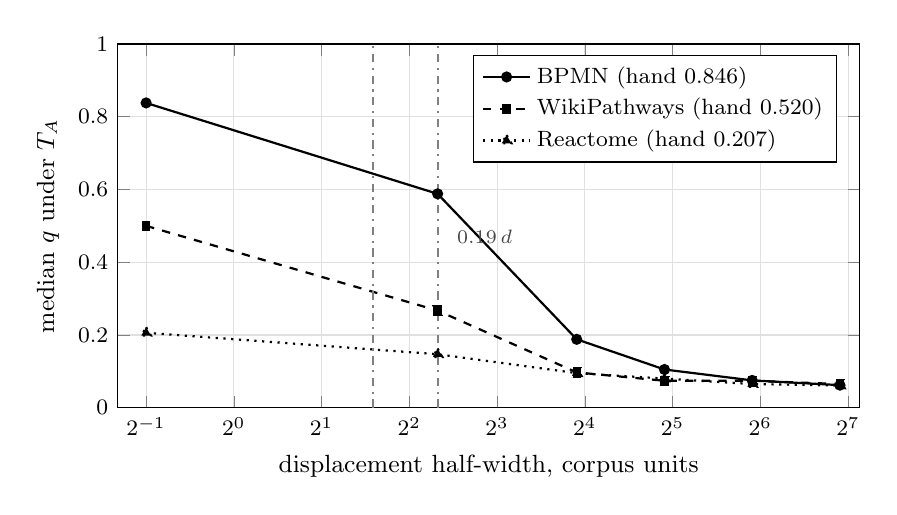
\begin{tikzpicture}
\begin{axis}[width=11cm,height=6.2cm,
  xmode=log,log basis x=2,
  xlabel={displacement half-width, corpus units},
  ylabel={median $q$ under $T_A$},
  ymin=0,ymax=1,xmin=0.4,xmax=140,
  legend pos=north east,legend cell align=left,
  grid=major,grid style={black!12},
  tick label style={font=\footnotesize},label style={font=\small},
  legend style={font=\footnotesize}]
\addplot[thick,mark=*,mark size=1.6pt] coordinates
  {(0.5,0.838)(5,0.588)(15,0.188)(30,0.105)(60,0.075)(120,0.062)};
\addlegendentry{BPMN (hand 0.846)}
\addplot[thick,mark=square*,mark size=1.5pt,dashed] coordinates
  {(0.5,0.500)(5,0.267)(15,0.097)(30,0.074)(60,0.074)(120,0.065)};
\addlegendentry{WikiPathways (hand 0.520)}
\addplot[thick,mark=triangle*,mark size=2pt,dotted] coordinates
  {(0.5,0.206)(5,0.147)(15,0.095)(30,0.080)(60,0.065)(120,0.061)};
\addlegendentry{Reactome (hand 0.207)}
\addplot[gray,thick,dash dot,forget plot] coordinates {(3,0)(3,1)};
\addplot[gray,thick,dash dot,forget plot] coordinates {(5,0)(5,1)};
\node[anchor=west,font=\scriptsize,gray!55!black] at (axis cs:5.4,0.47) {$0.19\,d$};
\end{axis}
\end{tikzpicture}
\caption{The displacement sweep, every box of every hand layout displaced by up to the
half-width, the alignment hold read at $d = 0.02$ and sixteen directions. The declared
half-pitch test sits at the left edge, 0.5 units, where nothing has changed: the corner of
$T_A$ releases a box only past $0.19\,d$, 3 units in the biological corpora and 5 in
BPMN. Past the bound the hold falls, BPMN 0.84 to 0.59 by a half-width of 5, and by 120
units every corpus is at the grid-snapped level of 0.06 to 0.09.}
\label{fig:sweep}
\end{figure}


\section{Reinsertion}\label{app:reinsert}

A constructive check of the recommendation (\texttt{reinsert.c},
\texttt{results/reinsert.md}; first-300 BPMN): delete each box in turn and let an energy
place it against the frozen rest, the distance to the person's position the score. Every
energy beats chance, 0.18 to 0.23 of the drawing width against 0.52 to 0.54, and adding
A1 to $C{+}O{+}L$ moves the median distance not at all: the neighbourhood is the distance
terms' choice. The rail is alignment's: with A1 offered, the box lands within 0.005 of the
person's row or column in 0.127, 0.101 and 0.226 of placements against 0.085, 0.083 and
0.162 without it, chance 0.02, McNemar $z$ 4.5 to 14.3 over placements and every
diagram-clustered interval excluding zero. Among placements within 0.05 of the true
position under both energies the rail rate rises from 0.41, 0.35 and 0.53 to 0.55, 0.46
and 0.67 while the near-stratum sizes barely move. The gain is stable under another seed,
twice the budget and the matched-budget uniform-sampling control.

\section{The plan and its outcomes}\label{app:plan}

The signed plan of 22 August 2026 fixed its hypotheses after a 60-diagram pilot the same
morning, so they carried no risk once the pilot had run; it is a plan, and the paper does
not claim a registration. Its hypotheses and what the run found:

\begin{center}\small
\begin{tabular}{@{}p{1cm}>{\raggedright\arraybackslash}p{7.6cm}>{\raggedright\arraybackslash}p{5.6cm}@{}}
\toprule
& hypothesis & outcome \\
\midrule
H1 & under $C{+}O$ the hand layout is held, median $q$ above 0.9 in every corpus & held: 1.00 \\
H2 & under $T_L$ alone it is not, median below 0.2 & held: 0.00; also true of every non-optimised layout \\
H3 & no positive weight on $T_L$ repairs $C{+}O{+}L$ & held: the step of Section~\ref{sec:results} \\
H4 & alignment holds more hand-placed boxes than orthogonality or node--edge separation, and more than the tool control & refuted on the held fraction: node--edge holds 0.88 to 1.00 against alignment's 0.21 to 0.85; held on the value against \texttt{neato} and on the hold against \texttt{neato}; below \texttt{dot} \\
H5 & under stress alone the hand layout is held less than \texttt{neato}'s & held: 0.00 against 1.00 \\
\bottomrule
\end{tabular}
\end{center}

Departures from the plan, all recorded after the analyses they concern: the plan's
primary alignment definition is gridiness, and the paper reports the gridiness value with
the A1 hold beside it because a step term's $q$ reads flatness; the flow term, declared
as an alternative, is measured as a criterion; the reading direction is fitted like $L$;
ELK, logged as unavailable, was obtained and run; the paired control is \texttt{dot}
rather than the registered \texttt{neato}, which the main table already separates from
the hand layouts on every distance term; the multiplicity family is the terms within one
corpus against one control; the BPMN sample is the random 300 of
Appendix~\ref{app:bpmn}; the radius in box widths, the A2 alignment definition and
containment as a hard constraint, all declared, were not run.

\begin{thebibliography}{99}
\bibitem{tdb88} R.~Tamassia, G.~Di Battista, C.~Batini. Automatic Graph Drawing and
 Readability of Diagrams. \emph{IEEE Transactions on Systems, Man, and Cybernetics}
 18(1):61--79, 1988.
\bibitem{dh96} R.~Davidson, D.~Harel. Drawing Graphs Nicely Using Simulated Annealing.
 \emph{ACM Transactions on Graphics} 15(4):301--331, 1996.
\bibitem{purchase02} H.~C. Purchase. Metrics for Graph Drawing Aesthetics. \emph{Journal
 of Visual Languages and Computing} 13(5):501--516, 2002.
\bibitem{kobourov} S.~G. Kobourov. Force-Directed Drawing Algorithms. In \emph{Handbook
 of Graph Drawing and Visualization}, CRC Press, 2013.
\bibitem{masui94} T.~Masui. Evolutionary Learning of Graph Layout Constraints from
 Examples. \emph{Proc.\ UIST '94}, 103--108, 1994.
\bibitem{spoenemann14} M.~Sp\"onemann, B.~Duderstadt, R.~von Hanxleden. Evolutionary Meta
 Layout of Graphs. \emph{Diagrams 2014}, LNCS, 16--30, 2014.
\bibitem{klammler19} M.~Klammler, T.~Mchedlidze, A.~Pak. Aesthetic Discrimination of Graph
 Layouts. \emph{Journal of Graph Algorithms and Applications} 23(3):525--552, 2019.
\bibitem{flud22} A.~Bharadwaj, D.~Gwizdala, Y.~Kim, K.~Luther, T.~M. Murali. Flud: A Hybrid
 Crowd--Algorithm Approach for Visualizing Biological Networks. \emph{ACM Transactions on
 Computer--Human Interaction} 29(1), 2022.
\bibitem{zhang26} P.~Zhang, X.~Li, X.~Wang, H.-W. Shen, Y.~Hu. Beauty in the Eye of AI:
 Aligning LLMs and Vision Models with Human Aesthetics in Network Visualization.
 arXiv:2604.03417, 2026.
\bibitem{ahuja01} R.~K. Ahuja, J.~B. Orlin. Inverse Optimization. \emph{Operations
 Research} 49(5):771--783, 2001.
\bibitem{keshavarz11} A.~Keshavarz, Y.~Wang, S.~Boyd. Imputing a Convex Objective Function.
 \emph{IEEE International Symposium on Intelligent Control}, 613--619, 2011.
\bibitem{chan19} T.~C.~Y. Chan, T.~Lee, D.~Terekhov. Inverse Optimization: Closed-Form
 Solutions, Geometry, and Goodness of Fit. \emph{Management Science} 65(3):1115--1135,
 2019.
\bibitem{odonovan14} P.~O'Donovan, A.~Agarwala, A.~Hertzmann. Learning Layouts for
 Single-Page Graphic Designs. \emph{IEEE Transactions on Visualization and Computer
 Graphics} 20(8):1200--1213, 2014.
\bibitem{gdcoll25} G.~J. Mooney, T.~Hegemann, A.~Wolff, M.~Wybrow, H.~C. Purchase.
 Universal Quality Metrics for Graph Drawings: Which Graphs Excite Us Most? In \emph{33rd
 International Symposium on Graph Drawing and Network Visualization} (GD 2025), LIPIcs 357,
 30:1--30:20, 2025.
\bibitem{ng00} A.~Y. Ng, S.~Russell. Algorithms for Inverse Reinforcement Learning. In
 \emph{Proc.\ 17th International Conference on Machine Learning} (ICML 2000), Morgan
 Kaufmann, 663--670, 2000.
\bibitem{ratliff06} N.~D. Ratliff, J.~A. Bagnell, M.~A. Zinkevich. Maximum Margin
 Planning. In \emph{Proc.\ 23rd International Conference on Machine Learning} (ICML 2006),
 729--736, 2006.
\bibitem{ziebart08} B.~D. Ziebart, A.~Maas, J.~A. Bagnell, A.~K. Dey. Maximum Entropy
 Inverse Reinforcement Learning. In \emph{Proc.\ 23rd AAAI Conference on Artificial
 Intelligence} (AAAI 2008), 1433--1438, 2008.
\bibitem{aswani18} A.~Aswani, Z.-J.~M. Shen, A.~Siddiq. Inverse Optimization with Noisy
 Data. \emph{Operations Research} 66(3):870--892, 2018.
\bibitem{smelser24} K.~Smelser, J.~Miller, S.~Kobourov. ``Normalized Stress'' is Not
 Normalized: How to Interpret Stress Correctly. \emph{2024 IEEE Evaluation and Beyond:
 Methodological Approaches for Visualization} (BELIV), 41--50, 2024.
\bibitem{ahmed24} R.~Ahmed, C.~Erten, S.~Kobourov, J.~Lotz, J.~Miller, H.~Taraz. Size
 Should Not Matter: Evaluating Network Visualizations with Stress. \emph{arXiv preprint
 arXiv:2408.04688}, 2024.
\bibitem{schulze14} C.~D. Schulze, M.~Sp\"onemann, R.~von Hanxleden. Drawing Layered Graphs
 with Port Constraints. \emph{Journal of Visual Languages and Computing} 25(2):89--106, 2014.
\bibitem{hola16} S.~Kieffer, T.~Dwyer, K.~Marriott, M.~Wybrow. HOLA: Human-like Orthogonal
 Network Layout. \emph{IEEE Transactions on Visualization and Computer Graphics}
 22(1):349--358, 2016.
\bibitem{ahmed20} R.~Ahmed, F.~De Luca, S.~Devkota, S.~Kobourov, M.~Li. Graph Drawing via
 Gradient Descent, (GD)$^2$. \emph{Graph Drawing (GD 2020)}, LNCS, 3--17, 2020.
\bibitem{kamada89} T.~Kamada, T.~Kawai. An Algorithm for Drawing General Undirected Graphs.
 \emph{Information Processing Letters} 31:7--15, 1989.
\bibitem{gansner05} E.~R. Gansner, Y.~Koren, S.~C. North. Graph Drawing by Stress
 Majorization. \emph{Graph Drawing (GD 2004)}, LNCS, 239--250, 2005.
\bibitem{agrawal24} A.~Agrawal, H.~Balc\i, H.~Hanspers et al. WikiPathways 2024: Next
 Generation Pathway Database. \emph{Nucleic Acids Research} 52(D1):D679--D689, 2024.
\bibitem{fabregat18} A.~Fabregat et al. Reactome Diagram Viewer: Data Structures and
 Strategies to Boost Performance. \emph{Bioinformatics} 34(7):1208--1214, 2018.
\bibitem{kunze11} M.~Kunze, A.~Luebbe, M.~Weidlich, M.~Weske. Towards Understanding
 Process Modeling: The Case of the BPM Academic Initiative. \emph{BPMN 2011}, LNBIP,
 44--58, 2011.
\bibitem{sola23} D.~Sola, C.~Warmuth, B.~Sch\"afer, P.~Badakhshan, J.-R. Rehse, T.~Kampik.
 SAP Signavio Academic Models: A Large Process Model Dataset. \emph{Process Mining
 Workshops (ICPM 2022)}, LNBIP, 453--465, 2023.
\bibitem{bohler16} A.~Bohler et al. Reactome from a WikiPathways Perspective. \emph{PLOS
 Computational Biology} 12(5):e1004941, 2016.
\bibitem{rome} G.~Di Battista, A.~Garg, G.~Liotta, R.~Tamassia, E.~Tassinari, F.~Vargiu.
 An Experimental Comparison of Four Graph Drawing Algorithms. \emph{Computational
 Geometry} 7(5--6):303--325, 1997.
\bibitem{ipsepcola06} T.~Dwyer, Y.~Koren, K.~Marriott. IPSep-CoLa: An Incremental
 Procedure for Separation Constraint Layout of Graphs. \emph{IEEE Transactions on
 Visualization and Computer Graphics} 12(5):821--828, 2006.
\bibitem{dunnart08} T.~Dwyer, K.~Marriott, M.~Wybrow. Dunnart: A Constraint-Based Network
 Diagram Authoring Tool. \emph{Graph Drawing (GD 2008)}, LNCS 5417, 420--431, 2009.
\bibitem{setcola18} J.~Hoffswell, A.~Borning, J.~Heer. SetCoLa: High-Level Constraints
 for Graph Layout. \emph{Computer Graphics Forum} 37(3):537--548, 2018.
\bibitem{marriott12} K.~Marriott, H.~Purchase, M.~Wybrow, C.~Goncu. Memorability of Visual
 Features in Network Diagrams. \emph{IEEE Transactions on Visualization and Computer
 Graphics} 18(12):2477--2485, 2012.
\bibitem{bennett07} C.~Bennett, J.~Ryall, L.~Spalteholz, A.~Gooch. The Aesthetics of Graph
 Visualization. \emph{Computational Aesthetics in Graphics, Visualization, and Imaging}
 (CAe 2007), Eurographics, 57--64, 2007.
\bibitem{vanham08} F.~van Ham, B.~Rogowitz. Perceptual Organization in User-Generated Graph
 Layouts. \emph{IEEE Transactions on Visualization and Computer Graphics} 14(6):1333--1339,
 2008.
\bibitem{dwyer09} T.~Dwyer, B.~Lee, D.~Fisher, K.~I. Quinn, P.~Isenberg, G.~Robertson,
 C.~North. A Comparison of User-Generated and Automatic Graph Layouts. \emph{IEEE
 Transactions on Visualization and Computer Graphics} 15(6):961--968, 2009.
\bibitem{purchase12} H.~C. Purchase, C.~Pilcher, B.~Plimmer. Graph Drawing Aesthetics:
 Created by Users, Not Algorithms. \emph{IEEE Transactions on Visualization and Computer
 Graphics} 18(1):81--92, 2012.
\bibitem{mooney25} G.~J. Mooney, J.~Miller, M.~Wybrow, S.~Kobourov, H.~C. Purchase.
 Stress in Graph Drawings: Perception, Preference, and Performance. In \emph{33rd
 International Symposium on Graph Drawing and Network Visualization} (GD 2025), LIPIcs 357,
 38:1--38:23, 2025.
\bibitem{pvw85} T.~Pavlidis, C.~J. Van Wyk. An Automatic Beautifier for Drawings and
 Illustrations. \emph{SIGGRAPH '85}, 225--234, 1985.
\bibitem{igarashi97} T.~Igarashi, S.~Matsuoka, S.~Kawachiya, H.~Tanaka. Interactive
 Beautification: A Technique for Rapid Geometric Design. \emph{UIST '97}, 105--114, 1997.
\bibitem{wageningen25} S.~van Wageningen, T.~Mchedlidze, A.~Telea. Same Quality Metrics,
 Different Graph Drawings. \emph{Graph Drawing (GD 2025)}, arXiv:2508.15557, 2025.
\bibitem{bergstra12} J.~Bergstra, Y.~Bengio. Random Search for Hyper-Parameter
 Optimization. \emph{Journal of Machine Learning Research} 13:281--305, 2012.
\bibitem{jw95} A.~Juels, M.~Wattenberg. Stochastic Hillclimbing as a Baseline Method for
 Evaluating Genetic Algorithms. \emph{Advances in Neural Information Processing Systems 8}
 (NIPS 1995), MIT Press, 430--436, 1996.
\end{thebibliography}

\end{document}
